\documentclass[../main.tex]{subfiles}

\usepackage{pgfplots}
\pgfplotsset{compat=1.15}
\usepackage{mathrsfs}
\usetikzlibrary{arrows}

\begin{document}

La introducción de los lenguajes libres de contexto aumenta ampliamente la clase de lenguajes que podemos describir formalmente; sin embargo, consideremos las siguientes oraciones presentadas en \cite{levy2012}: ''Ayer una mujer llegó que conocía'', ''Ayer un mujer y un hombre llegaron a los que cononocía y admiraba''. Notemos que la concordancia entre los sujetos ''hombre y mujerr' y el verbo ''llegaron'' y el pronombre relativo 'los que' marca la estructura de oración $xa^ib^ic^id^i$, el cual no es un lenguaje regular. \\
En este capítulo daremos por terminado el estudio de la jerarquía de Chomsky por medio de la teoría de categorías, presentando los lenguajes recursivamente enumerables que permiten representar oraciones como las anteriores, los cuales son comúnmente definidos de la siguiente forma:
\begin{itemize}
    \item son los lenguajes producidos por una gramática de tipo 0, las cuales son las gramáticas generativas cuyas reglas de producción tienen cero restricciones; y
    \item son los lenguajes reconocidos por una máquina de Turing 
\end{itemize}
En esta ocasión, las categorías adecuadas para trabajar los lenguajes recursivamente enumerables son las categorías monoidales que, como su nombre lo indica, son categorías dotadas de una operación binaria que cumple propiedades análogas a la estructura de un monoide algebraico. Además, tienen asociado un cálculo gráfico, es decir, existen diagramas que nos permiten representar los morfismos en la categoría y, más aún, nos permiten efectuar operaciones en ellos mediante deformaciones. Estos diagramas nos permitirán definir las categorías monoidales libres de forma combinatoria. \\
Finalmente, mostraremos que los lenguajes generados por una categoría monoidal son exactamente los lenguajes recursivamente enumerables. 

\section{Categorías monoidales}

\begin{dfn}
	Una \textbf{signatura monoidal} $G$ es una signatura de la siguiente forma: 
	$$\signature{G_1}{G_0^*}$$
    Un \textbf{morfismo de signaturas monoidales} \( \phi:G \to \Gamma\) es un par de funciones \( \phi_0: G_0 \to \Gamma_0\) y \( \phi_1: G_1 \to \Gamma_1\) tales que el siguiente diagrama conmuta: 
	\[
	\begin{tikzcd}
		G_0^* \arrow{d}{\phi_0} & G_1 \arrow{r}{\tt{dom}} \arrow{l}{\tt{cod}} \arrow{d}{\phi_1} & G_0^* \arrow{d}{\phi_0} \\
		\Gamma_0^* & \Gamma_1 \arrow{r}{\tt{dom}} \arrow{l}{\tt{cod}} & \Gamma_0^*
	\end{tikzcd}
	\]
	Con tales morfismos, las signaturas monoidales forman la categoría \textbf{MonSig}.	
\end{dfn}

\begin{dfn}
	Una \textbf{categoría monoidal estricta} $(\mathcal{C}, \otimes, 1)$ es una categoría $\mathcal{C}$ con un bifuntor\footnote{Un bifuntor es un funtor en cada entrada} $\otimes : \mathcal{C} \times \mathcal{C} \to \mathcal{C}$ y un objeto distinguido $1$ en $\mathcal{C}$ en la que se satisfacen las siguientes ecuaciones:
	\begin{enumerate}
		\item $1 \otimes f = f = f \otimes 1$
		\item $f \otimes (g \otimes h) = (f \otimes g) \otimes h$
	\end{enumerate} 
	para cualesquiera $f, g, h$ morfismos en $\mathcal{C}$.\\
	Un funtor monoidal estricto es un funtor entre categorías monoidales $F : \mathcal{C} \to \mathcal{D}$ que preserva el producto tensorial, es decir, $F(g \otimes_{\mathcal{C}} f) = F(g) \otimes_{\mathcal{D}} F(g)$. A la categoría de categorías monoidales con morfismos los funtores monoidales la denotamos $\textbf{MonCat}$
\end{dfn}
Notemos que en una categoría monoidal nuestros morfismos pueden componerse de dos maneras. Dado $f:A \to B$ y $g: B \to C$ morfismos podemos construir la composición $g \circ f: A \to C$. Pero también dados $u: A \to C$ y $v: B \to D$ podemos usar nuestro funtor para formar el morfismo $u \otimes v : A \otimes B \to C \otimes D$. \\
Es usual interpretar ambas composiciones de la siguiente manera: la composición usual es secuencial, es decir, primero se ejecuta el primer morfismo y después aplicamos el segundo; y la composición monoidal es paralela, es decir, ejecutamos ambos morfismos de manera simultánea. \\
Las consideraciones anteriores motivan un lenguaje gráfico para categorías monoidales mediante cables y cajas. Definimos recursivamente el lenguaje gráfico de la siguiente manera: Sean $A,B,C,D$ objetos y $f:A \to B$, $g:B \to C$ y $h:C \to D$ morfismos en una categoría monoidal, tenemos la siguiente representación gráfica. Estos diagramas son llamados \textbf{diagramas de cables}.
\begin{figure}[H]
	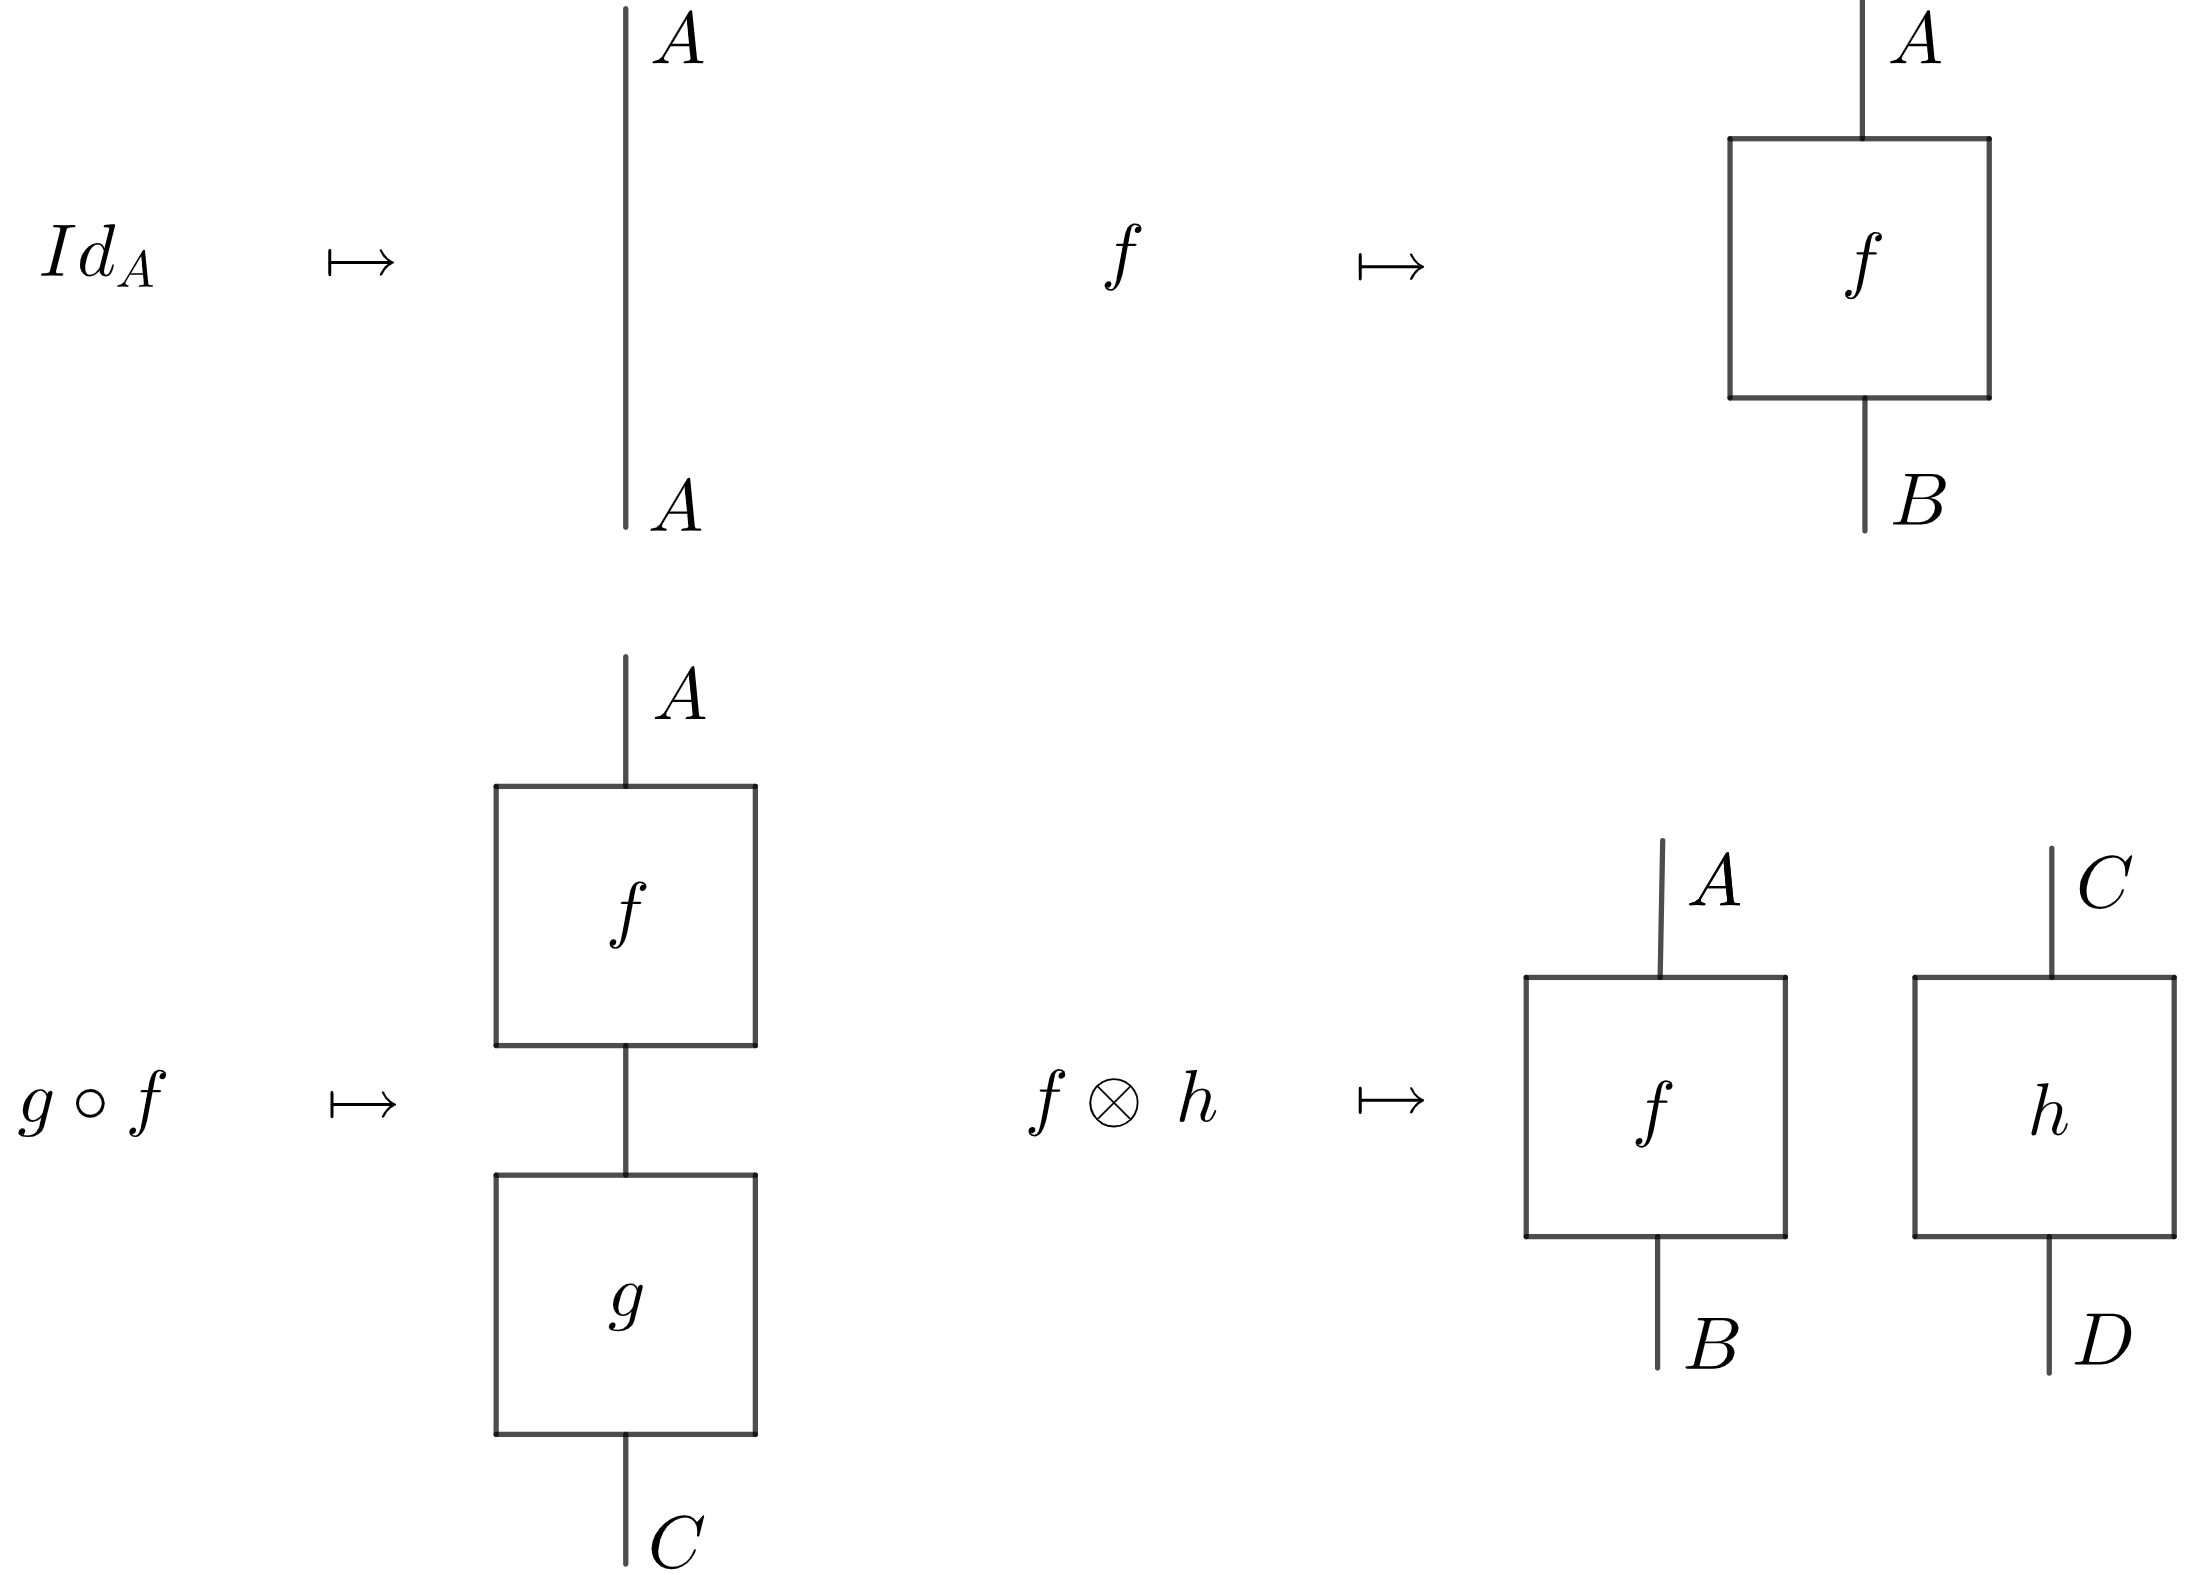
\includegraphics[scale=2.9]{diagrama/lenguaje.png}
	\centering
	\caption{Lenguaje gráfico para categorías monoidales}
	\label{lenguaje}
\end{figure}
Como es de esperarse, las dos operaciones entre los morfismos de nuestra categorías se ''comportan bien'' entre sí, como veremos en la siguiente proposición. 
\begin{prop}
	Sea $(\mathcal{C},\otimes , 1)$ una categoría monoidal y sean $f:A \to B$, $g:B \to C$, $h:D \to E$ y $j:E \to F$ morfismos de $\mathcal{C}$, entonces
	
	\begin{equation} \label{intLaw1}
		(g\circ f) \otimes (j \circ h) = (g \otimes j) \circ (f \otimes h)
	\end{equation}
	
	\begin{equation} \label{intLaw2}
		 (Id_B \otimes h) \circ (f \otimes Id_D) = f \otimes h = (f \otimes Id_E) \circ (Id_A \otimes h) 
	\end{equation} 
	 
\end{prop} 

\begin{proof}
	Sean $f:A \to B$, $g:B \to C$, $h:D \to E$ y $j:E \to F$ morfismos en una categoría monoidal $\mathcal{C}$. \\
	Primero probemos \ref{intLaw1}.
	\begin{align*}
		(g\circ f) \otimes (j \circ h) &= \otimes (g\circ f, j \circ h) \\
		&= \otimes ((g,j)) \circ (f,h))\\
		&=(\otimes (g,j)) \circ (\otimes (f,h)) & \text{por la bifuntorialidad de $\otimes$}\\
		&=(g \otimes j) \circ (f \otimes h)
	\end{align*}
	Ahora, veamos  \ref{intLaw2}
	\begin{align*}
		(Id_B \otimes h) \circ (f \otimes Id_D) &= (Id_B \circ f) \otimes (h \circ Id_D)	& \text{Por \ref{intLaw1}}\\
		&=f \otimes h \\
		&=(f \circ Id_A) \otimes (Id_E \circ h) \\
		&= (f \otimes Id_E) \circ (Id_A \otimes h) & \text{Por \ref{intLaw1}} 
	\end{align*}
\end{proof}
Podemos expresar en el lenguaje gráfico de categorías monoidales la ecuación \ref{intLaw2} de la siguiente forma:
\begin{figure}[H]
	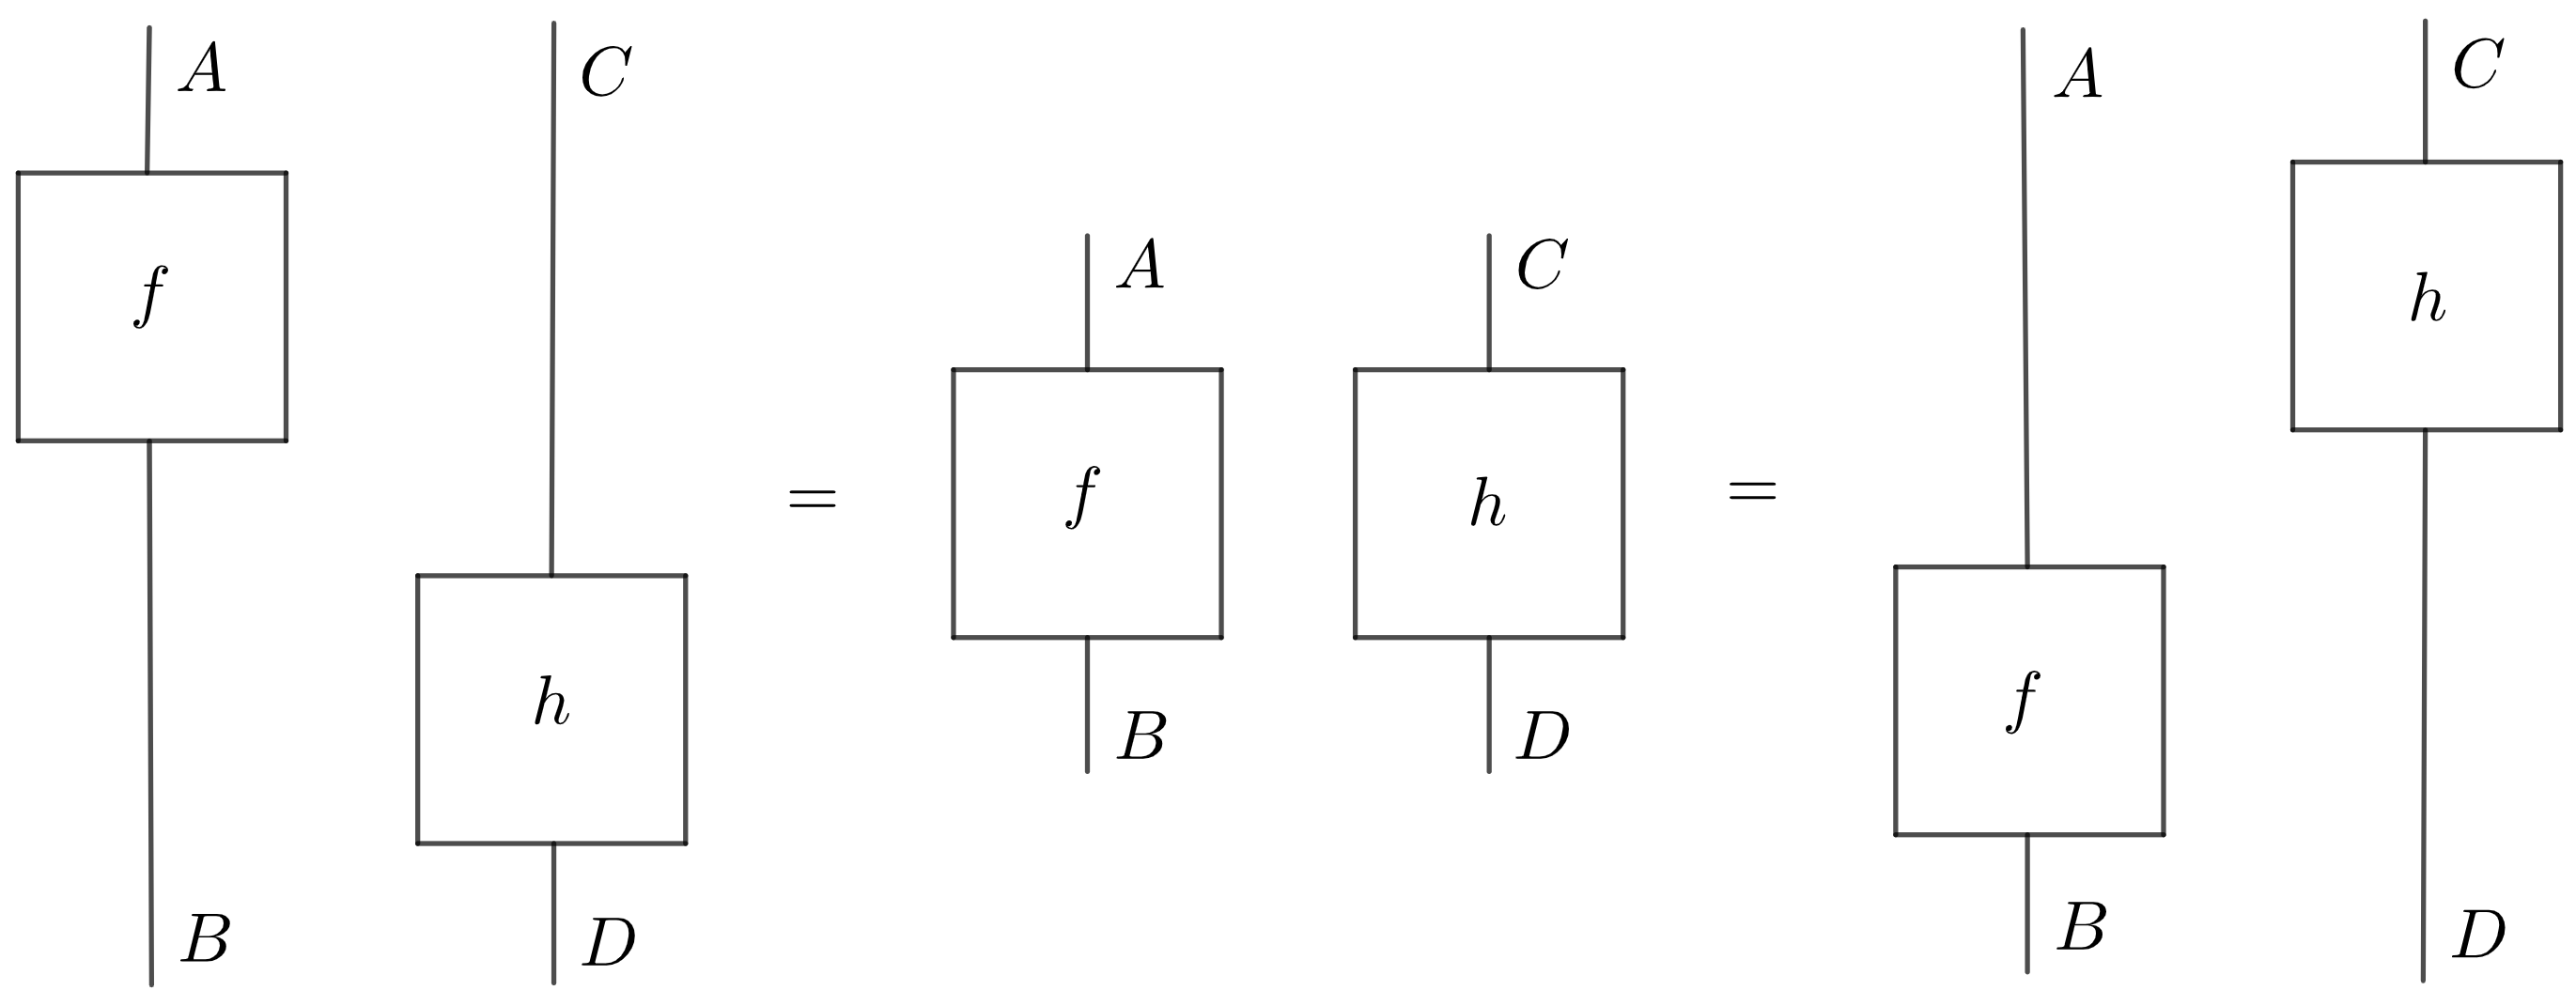
\includegraphics[scale=2.9]{diagrama/intercambio.png}
	\centering
	\label{intercambio}
\end{figure}
\noindent La ecuación anterior sugiere que siempre podemos encontrar diagramas donde cada caja este en un nivel distinto al resto, así que probémoslo, pero antes veamos la siguiente definición para poder enunciar nuestra proposición.

\begin{dfn}
	Un diagrama de cables está en \textbf{posición general} si no hay otra caja a la derecha o a la izquierda de cada caja.
\end{dfn}

\begin{prop}
	Todo diagrama de cables es equivalente a un diagrama de cables en posición general. 
	\label{posgeneral}
\end{prop}
\begin{proof}
	Sea $D$ un diagrama de cables. Haremos la demostración por inducción sobre el número de cajas en el diagrama. \\
	La base de inducción es trivial, pues si $D$ tiene una caja ya acabamos. \\
	Supongamos que el resultado es cierto para algún $n$ y que $D$ tiene $n+1$ cajas. \\
	Sea $f$ la caja ubicada más a la derecha y abajo en el diagrama y consideremos $D'$ el diagrama obtenido al sustituir $f$ por $id_{dom(f)}$. Entonces $D'$ tiene $n$ cajas y por hipótesis es equivalente a un diagrama de cajas $G'$ en posición general; consideremos ahora el diagrama $G$ que se obtiene al pegarle $f$ en el cable al que se lo habíamos cortado. \\ 
    Observemos que la caja que colocamos sigue siendo la más derecha y abajo, y a su  izquierda hay a lo más una caja $g$ (si no, ya acabamos), pues $G'$ está en posición general. Entonces basta hacer la siguiente deformación o, en otras palabras, aplicar \ref{intLaw1}.
	
	\begin{figure}[H]
		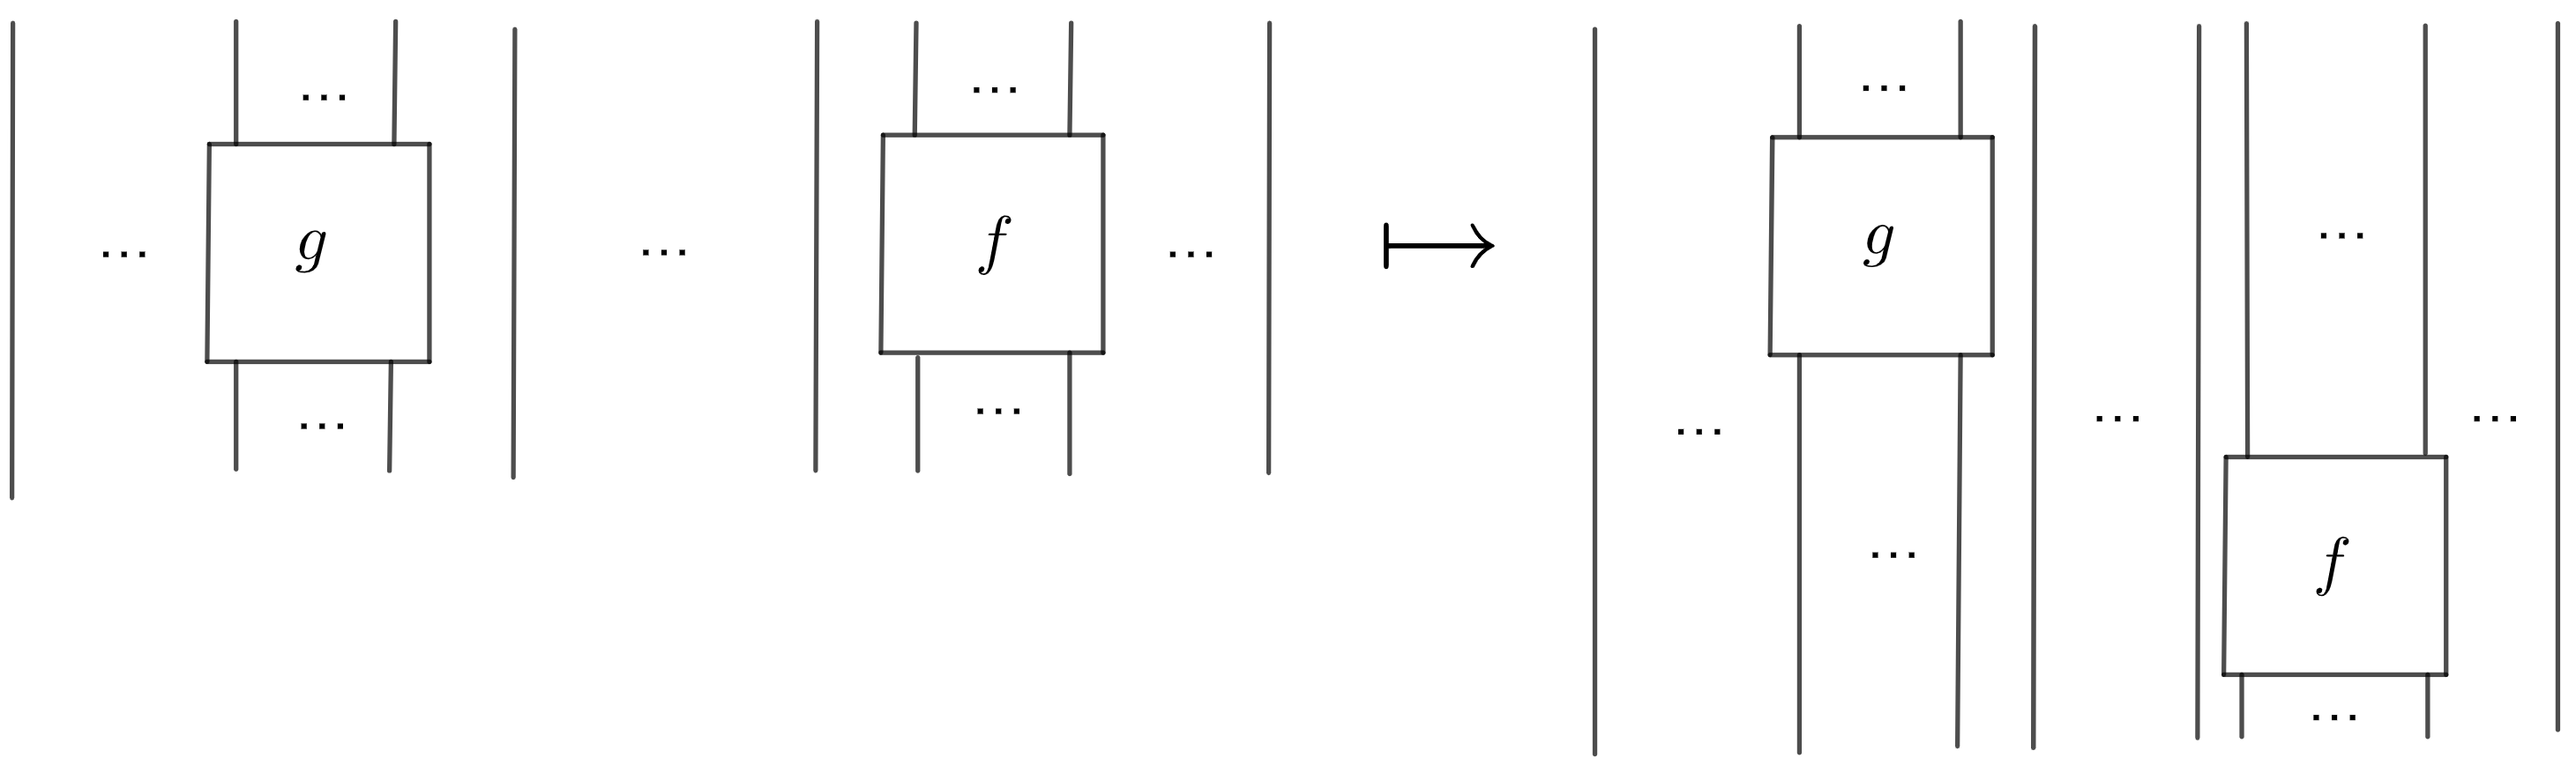
\includegraphics[scale=5]{diagrama/formagen.png}
		\centering
	\end{figure}
\end{proof}
\noindent Notemos que el argumento de la prueba anterior fue expresado de dos formas distintas, por medio de la igualdad \ref{intLaw1} y por su representación en el diagrama de cables. Sin embargo, es válido si el lector considera que fue una coincidencia muy afortunada y tenga sus reservas. Sin embargo, el siguiente teorema debido a A. Joyal y R. Street  nos iluminará en el uso de diagramas de cables, cuya demostración puede consultarse en \cite{joyal88} 
\begin{thm}[Teorema de coherencia del cálculo gráfico en categorías monoidales]
    Una ecuación $f=g$ bien formada\footnote{Una ecuación entre morfismos es bien formada si los morfismos efectivamente son parte la categoría y poseen tanto el mismo dominio como codominio } entre morfismos de una categoría monoidal es válida en la categoría monoidal si y sólo si los diagramas de cables de $f$ y $g$ son equivalentes salvo isotopías planas. \\
    Dos diagramas de cables son equivalentes salvo isotopías planas si es posible transformar uno en el otro moviendo continuamente las cajas y cables sin permitir que estos se crucen entre sí.
\end{thm}


\noindent La proposición y teorema anterior serán fundamentales en nuestro objetivo: generar una categoría monoidal libre a partir de una signatura monoidal. Para ello, primero describiremos un lenguaje gráfico para las signaturas monoidales ya que lo usaremos en la descripción de categorías monoidales.\\
Sea $G$ una signatura monoidal y sea $f: \vec{a} \to \vec{b} \in G_1$. Diremos que $f$ es una caja y la representaremos como:  
 
 \begin{center}
 	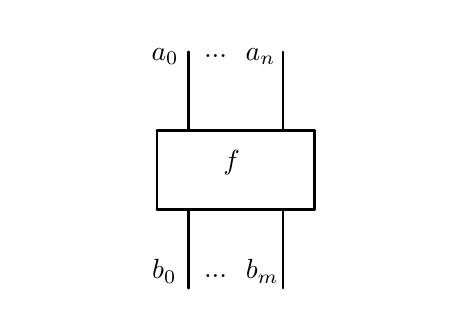
\begin{tikzpicture}[line cap=round,line join=round,>=triangle 45,x=2cm,y=2cm]
 		\clip(0.17821673525377257,-0.06342935528120883) rectangle (2.754019204389575,1.6537722908093206);
 		\draw [line width=1pt] (1,1)-- (2,1);
 		\draw [line width=1pt] (1,0.5)-- (2,0.5);
 		\draw [line width=1pt] (1,1)-- (1,0.5);
 		\draw [line width=1pt] (2,1)-- (2,0.5);
 		\draw (1.3580932784636492,0.9391632373113798) node[anchor=north west] {$f$};
 		\draw [line width=1pt] (1.2,1)-- (1.2,1.5);
 		\draw [line width=1pt] (1.8,1)-- (1.8,1.5);
 		\draw [line width=1pt] (1.2,0.5)-- (1.2,0);
 		\draw [line width=1pt] (1.8,0.5)-- (1.8,0);
 		\draw (1.2359533607681759,1.543319615912201) node[anchor=north west] {$...$};
 		\draw (0.9025377229080936,1.5853772290809255) node[anchor=north west] {$a_0$};
 		\draw (1.5004389574759947,1.5853772290809255) node[anchor=north west] {$a_n$};
 		\draw (0.9067764060356655,0.2421673525377199) node[anchor=north west] {$b_0$};
 		\draw (1.5009327846364887,0.2421673525377199) node[anchor=north west] {$b_m$};
 		\draw (1.2359533607681759,0.1473525377229054) node[anchor=north west] {...};
 	\end{tikzpicture}
 	
 \end{center}

Además, tenemos dos casos distinguidos que corresponden a morfismos de la forma $u: \varepsilon \to a$ y $w: b \to \varepsilon$ cuya representación es la siguiente.
\[
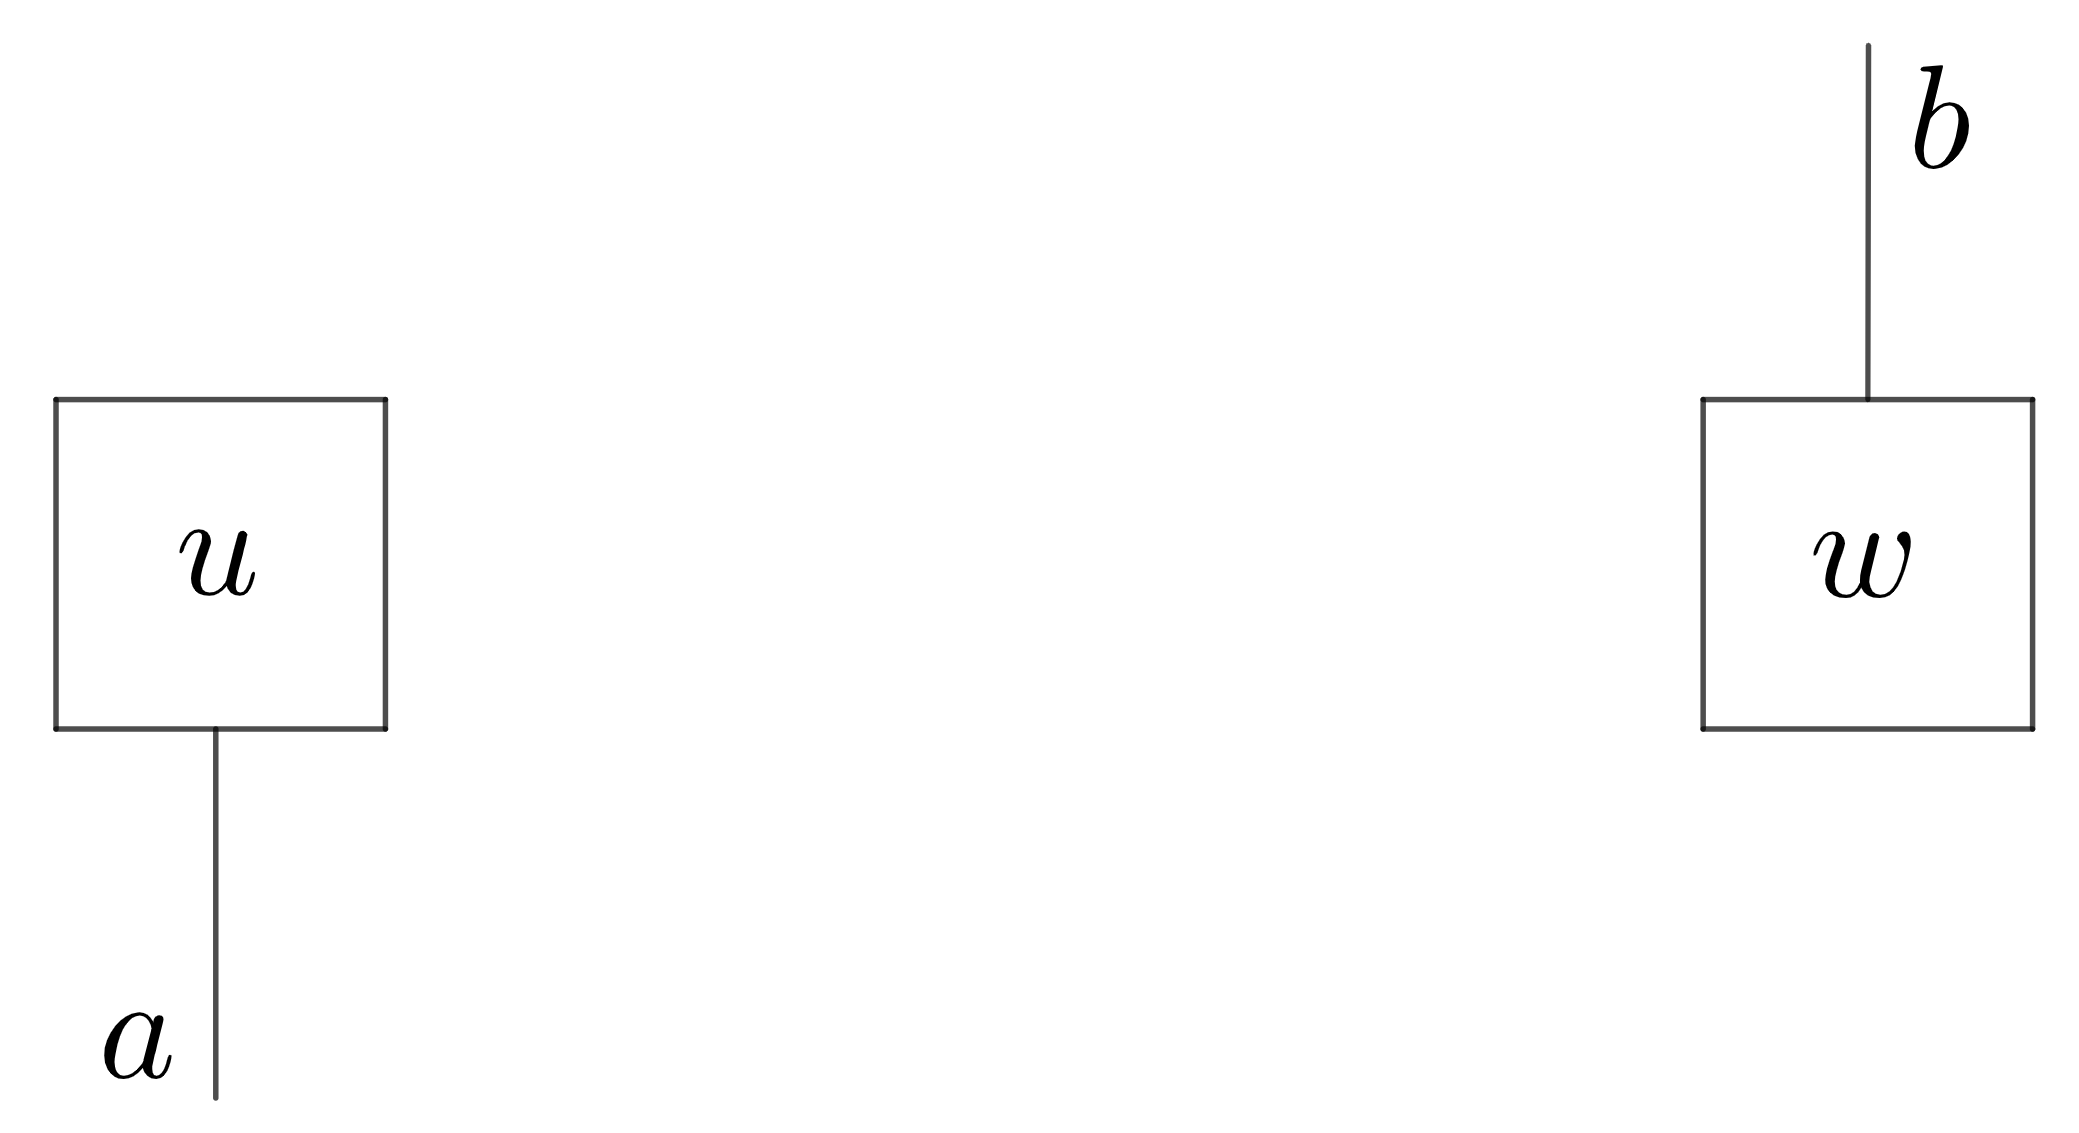
\includegraphics[scale=.5]{diagrama/estadoEfecto.png}
\]
Usaremos la descripción anterior para construir la categoría monoidal libre $\textbf{MC}(G)$ asociada a una signatura monoidal; para ello, primero veamos qué es una signatura de niveles. \\
Dada $G$ una signatura monoidal definimos la \textbf{signatura de niveles} de $G$ como
\[
\begin{tikzcd}
	G_0^* & L(G)=G_0^* \times G_1 \times G_0^* \arrow{r}{\tt{dom}} \arrow{l}{\tt{cod}}  & G_0^* 
\end{tikzcd}
\]
donde para cada nivel $l=(u, f:x \to y, v)$ en $L(G)$ definimos ${\tt{dom}} (l)=uxv$ y  ${\tt{cod}}(l)=uyv$, gráficamente representamos a $l$ de la siguiente manera
\[
	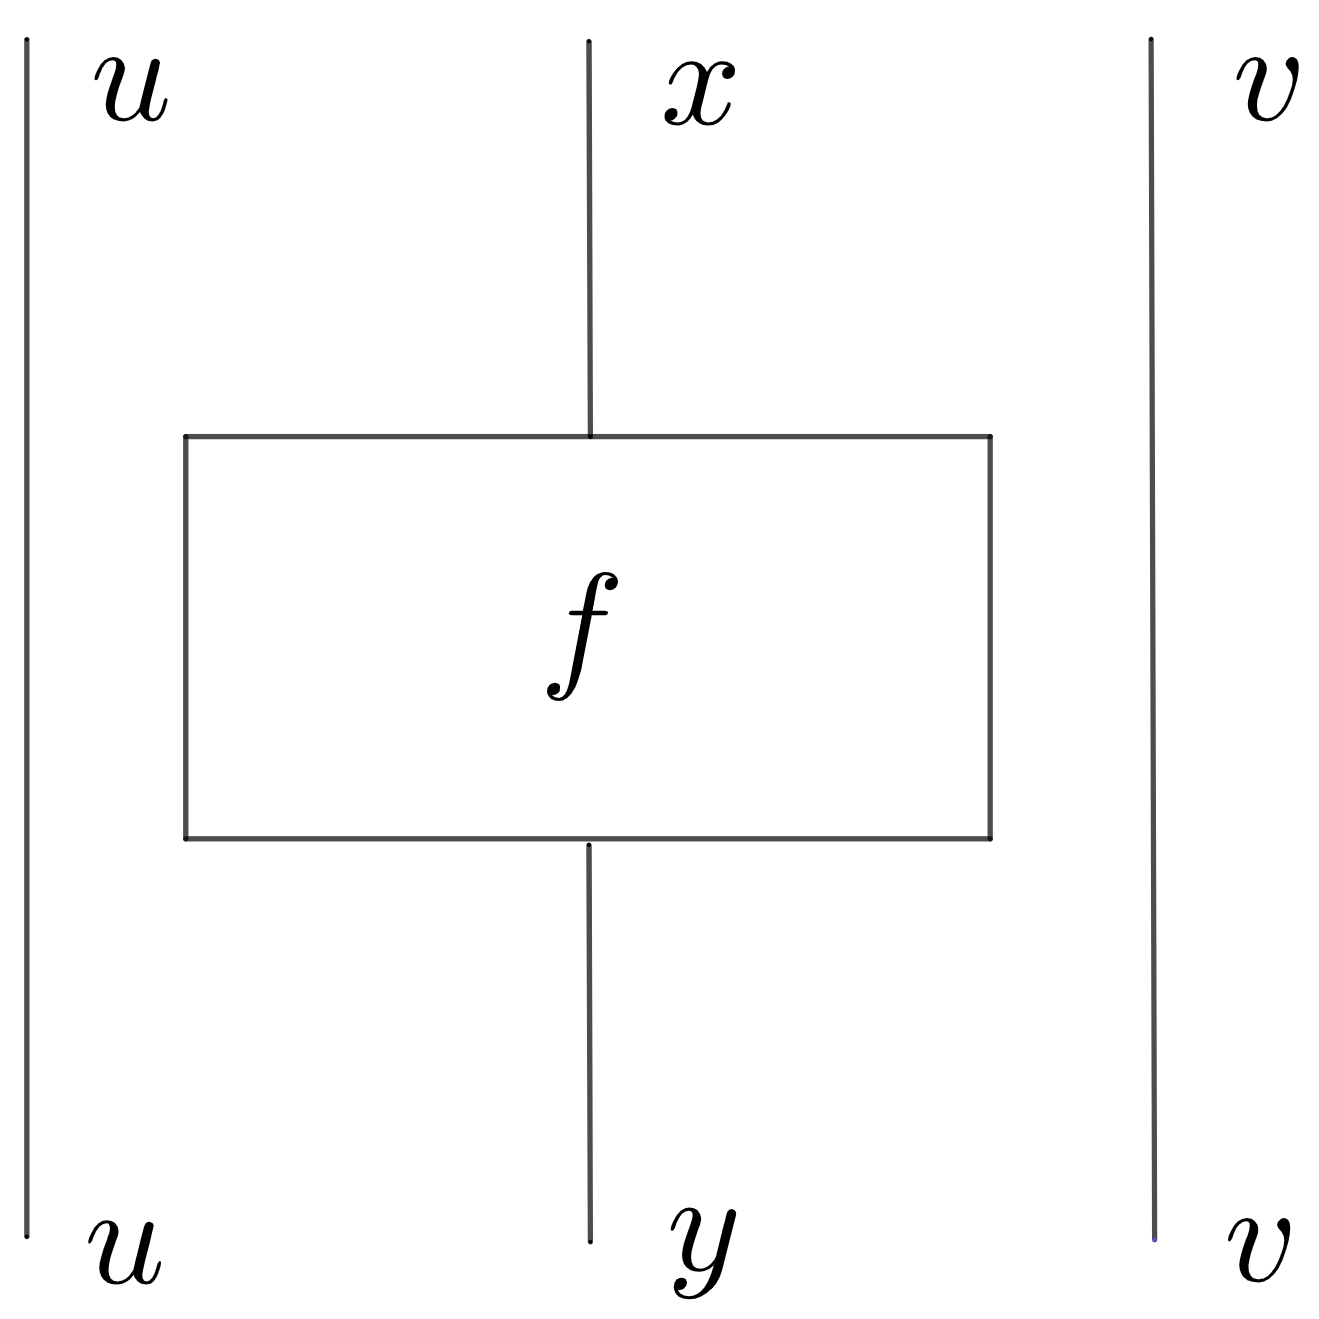
\includegraphics[scale=2.3]{diagrama/layer.png}
\]
Sea $\textbf{PMC}(G)$, la categoría libre cuyos objetos son los diagramas premonoidales y el conjunto de morfismos generadores son secuencias de niveles de la forma $(d_1, \dots , d_n)$ tales que ${\tt{cod}}(d_i)={\tt{dom}}(d_{i+1})$ para cada $i \in \{ 1,...,n-1 \}$. \\
Veamos el siguiente ejemplo de un diagrama premonoidal generado con la signatura $G_0=\{ a, b, c, u, v, y, x \}$ y $G_1=\{ f: c \to xv , g: b \to u, h: x \to y \}$
\[
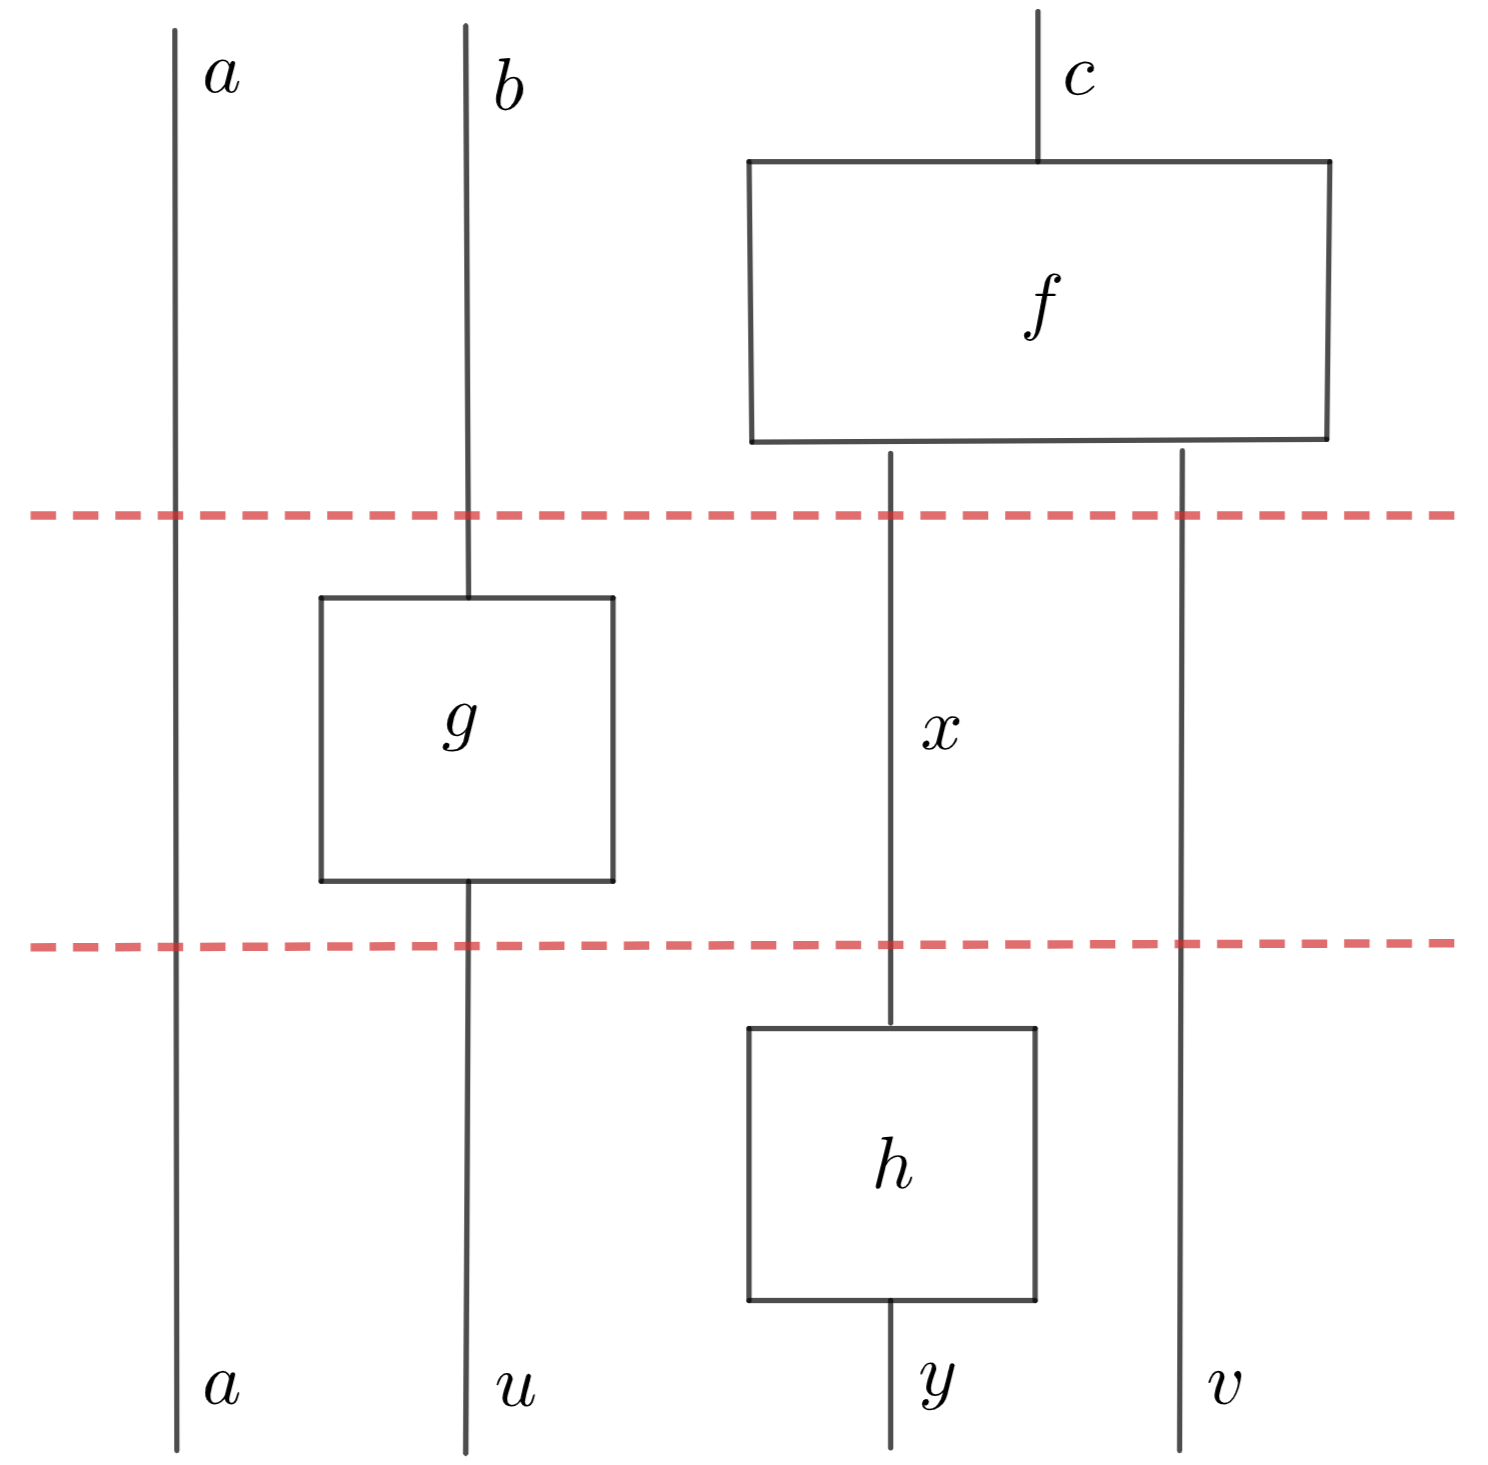
\includegraphics[scale=2.7]{diagrama/premonoidal.png}
\]
Supongamos que queremos construir el diagrama a partir de la signatura, ¿qué información necesitamos? En principio, conocer el número de niveles que conforma el diagrama, en nuestro caso tres, luego conocer el dominio y codominio del diagrama, $abc$ y $auyv$ respectivamente, además de la lista de cajas en cada nivel, $[f,g,h]$. Finalmente, necesitamos conocer la posición en la que se encuentra la caja en cada nivel, lo cual lo identificamos señalando el número de cables a la izquierda de la caja, $(2,1,2)$.  \\
Aunque la última condición es innecesaria en el diagrama anterior, es importante en casos como el siguiente, donde los primeros datos no determinan un único diagrama premonoidal. 
\[
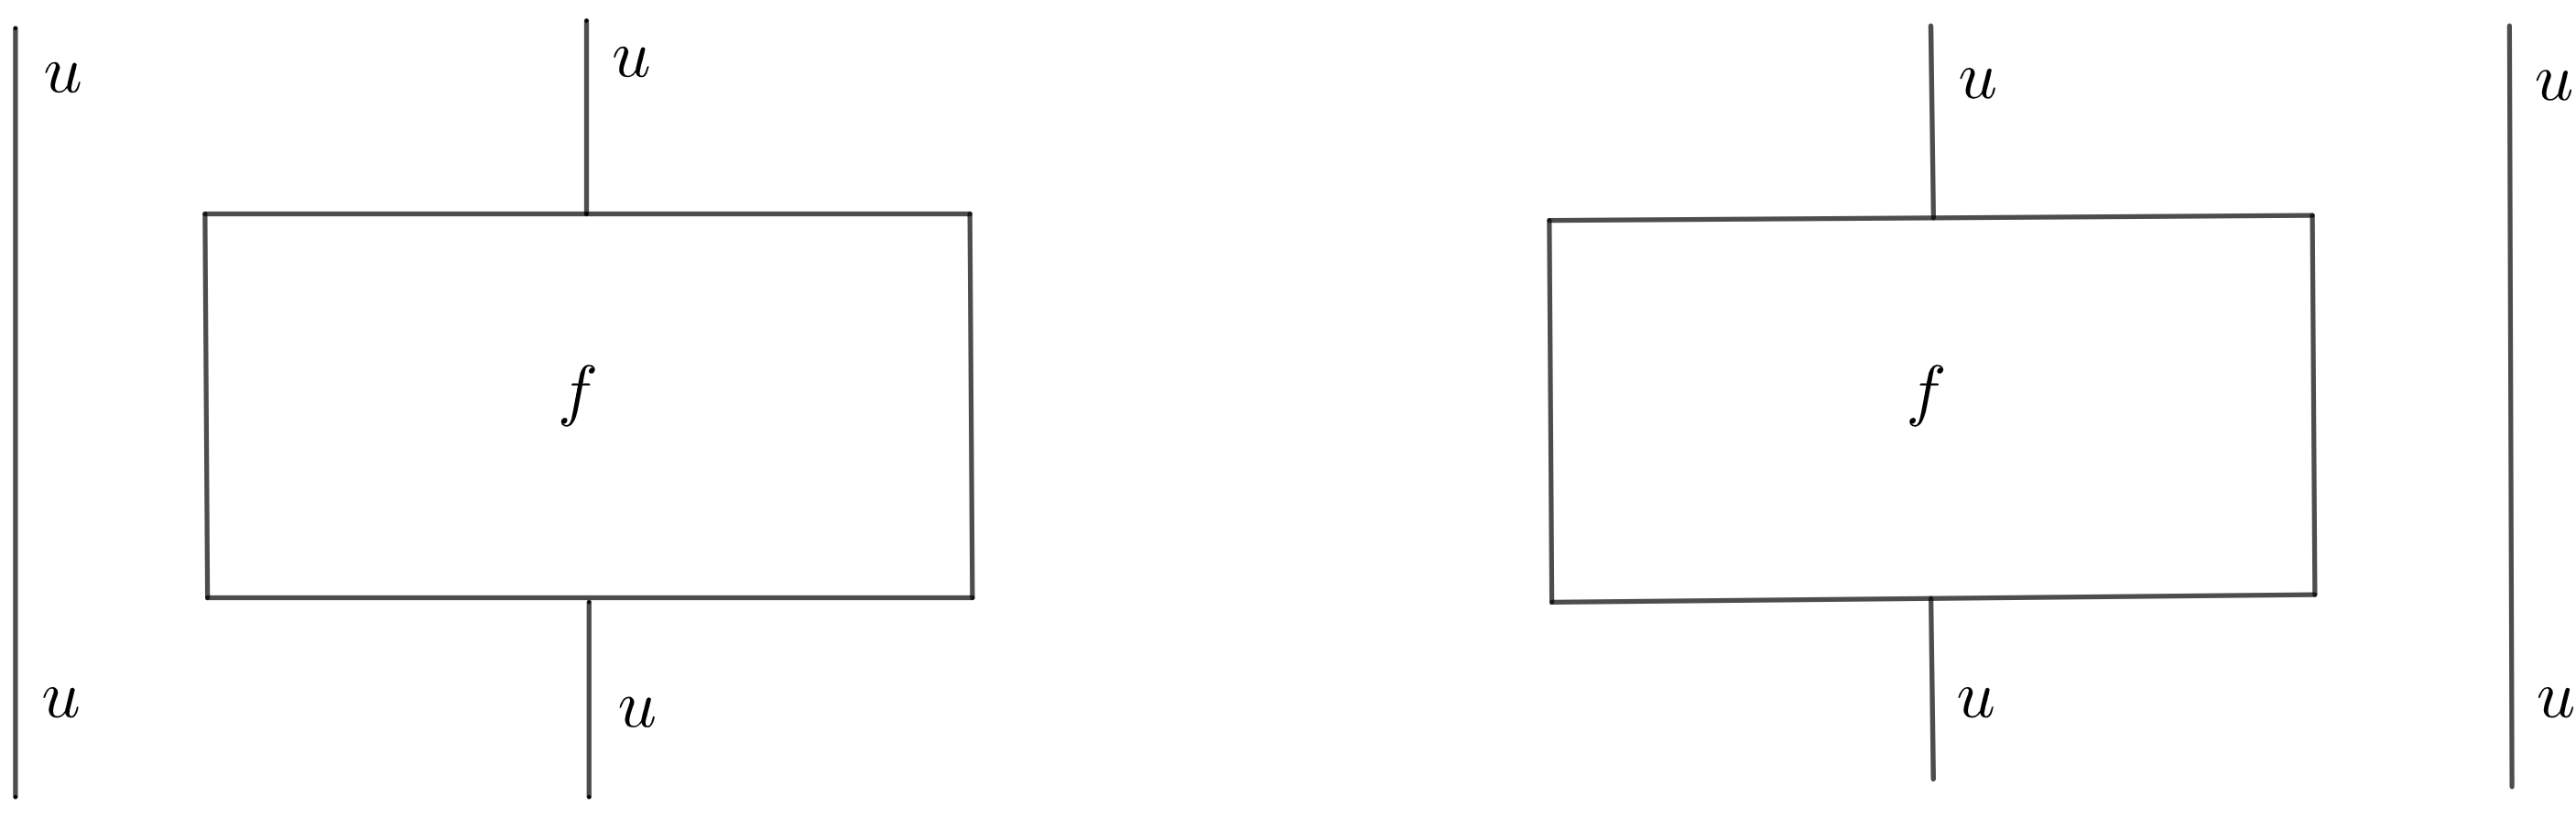
\includegraphics[scale=3.6]{diagrama/premonoidal2.png}
\]
La explicación anterior motiva nuestra siguiente proposición, una manera eficiente de representar la información contenida en un diagrama premonoidal:

\begin{prop}[Codificación de diagramas premonoidales]
\label{decode}
	Sea $G$ una signatura monoidal. Un diagrama premonoidal $d$ en $\textbf{PMC}(G)$ está únicamente determinada de la siguiente forma:
	\begin{enumerate}
		\item \textit{un dominio}: ${\tt{dom}}(d) \in G_0^*$
		\item \textit{un codominio}: ${\tt{cod}}(d) \in G_0^*$
		\item \textit{una lista de cajas}: ${\tt{cajas}}(d) \in G_1^n$
		\item \textit{una lista de números identificadores}: ${\tt{id}}(d) \in \mathbb{N}^n$
	\end{enumerate}
	donde $n$ es el número de niveles del diagrama $d$ y el $n-$ésimo identificador señala la posición de la caja en el $n-$ésimo nivel, indicando el número de ''cables'' a la izquierda de la caja. \\
	Más aún, la información anterior define un diagrama premonoidal válido si para cada $\i \in \{ 1, ..., n\}$ tenemos que
	$${\tt{peso}}(d)_i \geq {\tt{id}}(d)_i + |{\tt{dom}}(b_i)|$$
	donde
	\begin{equation*}
		{\tt{peso}}(d)_1 = 	|{\tt{dom}}(d)| \quad \quad  {\tt{peso}}(d)_{i+1}= {\tt{peso}}(d)_i + |{\tt{cod}}(b_i)| - |{\tt{dom}}(b_i)| 
	\end{equation*}
	con $b_i={\tt{boxes}}(d)_i$
\end{prop}
Notemos que la función $\tt{peso}$ indica el número de cables con los que inicia cada nivel; así, la desigualdad significa que este número debe ser mayor que el número de cables que estarán a la izquierda de la caja menos el número de cables que necesita la caja del nivel. Bajo estas condiciones, es evidente que el diagrama generado será válido.  \\
Ahora bien, notemos que los elementos de $\textbf{PMC}(G)$ se parecen mucho a diagramas de cables en posición general; sin embargo, necesitamos establecer cuándo dos diagramas premonoidales son equivalentes. Para ello, veamos las siguientes definiciones.
\begin{dfn}
	Sea $G$ una signatura y $d$ un diagrama premonoidal de $G$. Decimos que $d$ admite un intercambio izquierdo en el nivel $n$ si ${\tt{id}}(d)_{n+1} \geq {\tt{id}}(d)_{n} + |cod(b_n)|$ y admite un intercambio derecho en el nivel $n+1$ si ${\tt{id}}(d)_{n} \geq {\tt{id}}(d)_{n+1} + |dom(b_n)|$.
\end{dfn}
En otras palabras, un intercambio es posible cuando las cajas a intercambiar no tienen cables en común. Ahora sí, veamos qué es un intercambio.

\begin{dfn}
	Sea $G$ una signatura y $d$ un diagrama premonoidal de $G$. Si $d$ admite un intercambio izquierdo (o derecho) en el nivel $n$, entonces generamos un nuevo diagrama idéntico en todos los niveles a $d$ salvo en $n$ y $n+1$ donde hay un cambio de la siguiente forma: 
	
	\begin{figure}[H]
		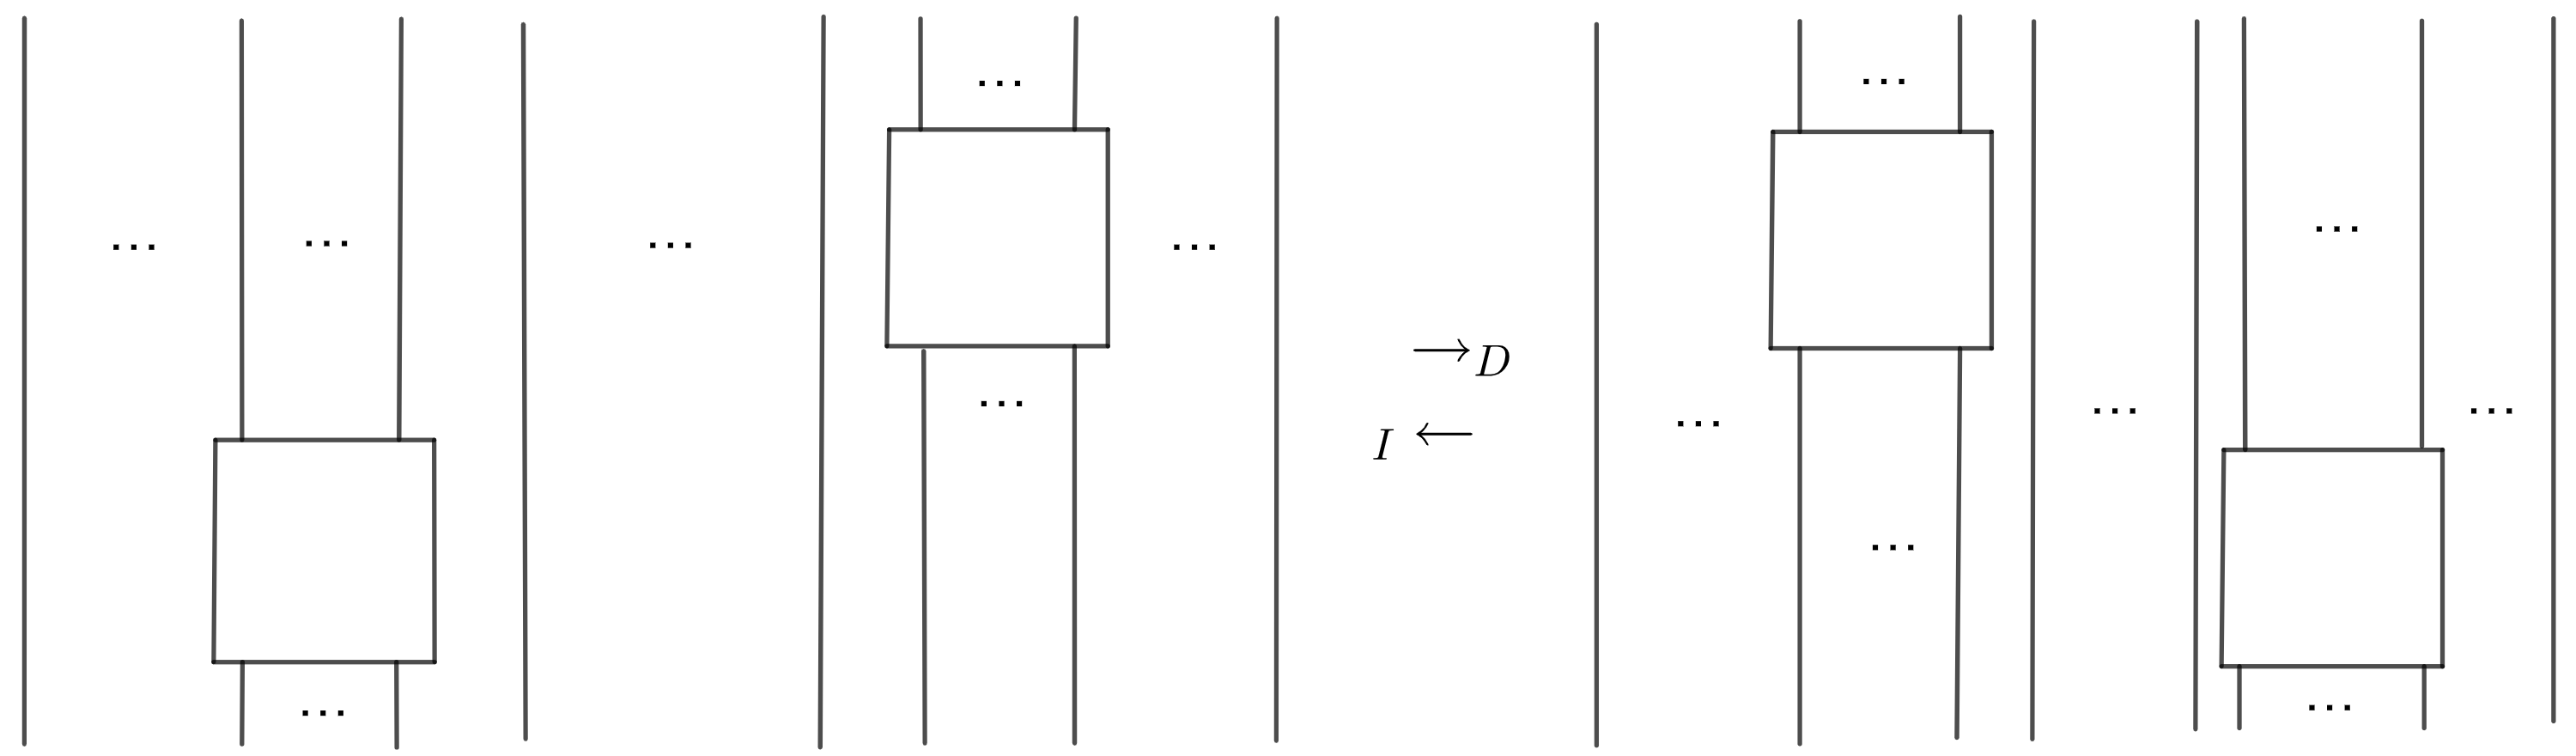
\includegraphics[scale=5]{diagrama/izqder.png}
		\centering
	\end{figure}	
Decimos que el nuevo diagrama es el \textbf{intercambio izquierdo (o derecho) en el nivel $n$ de $d$}.
\end{dfn}
Claramente los diagramas producidos tras un intercambio son también un diagrama válido. Definimos una reducción de diagramas como una secuencia de intercambios izquierdos o derechos. Con ello, definimos la siguiente relación: dos diagramas $d$ y $d'$ están $\sim$-relacionados si existe una reducción que lleve $d$ a $d'$. 

\begin{prop}
	Sea $G$ una signatura monoidal. La relación $\sim$ sobre el conjunto de diagramas premonoidales de $G$ es de equivalencia. 
	\label{equiv}
\end{prop}
\begin{proof}
	Sea $G$ una signatura monoidal.
	Sea $d$ una diagrama premonoidal. Consideramos la secuencia de reducciones vacía, entonces $d \sim d$. Por lo tanto, $\sim$ es reflexiva.\\
	Sea $d$ y $d'$ diagramas tales que $d \sim d'$. Sea $p_1^{r_1}, p_2^{r_2}, ... , p_n^{r_n}$ la secuencia de reducciones que lleva $d$ a $d'$ con $r_i \in \{ d, i\}$ para todo $i \in \{1, ...,n \}$, es decir, indica si el intercambio fue izquierdo o derecho. Notemos que un intercambio izquierdo es el inverso del derecho y viceversa, entonces consideremos $r'_{i}$ como el opuesto a $r_{i}$. Entonces la reducción $p_n^{r'_n}, p_{n-1}^{r'_{n-1}}, ... , p_1^{r'_1}$ lleva $d'$ a $d$. Por lo tanto, $d' \sim d$, así tenemos que $\sim$ es simétrica. \\  
	Por último, sean $d$, $d'$ y $d''$ tales que $d \sim d'$ y $d' \sim d''$. Entonces hay una reducción que lleva $d$ a $d'$ y una que lleva $d'$ a $d''$, así hay una reducción que lleva $d$ a $d''$, es decir, $d \sim d''$. Por lo tanto, $\sim$ es transitiva. \\
	Por lo tanto, $\sim$ es de equivalencia. 
\end{proof}
Otra forma de expresar la proposición anterior es señalando que cualesquiera dos diagramas premonoidales tales que pueda deformarse, sin cruzar o cortar cables, uno en el otro están $\sim$-relacionados. Con todo lo anterior, ya estamos en condiciones de conocer a nuestra categoría monoidal libre, \textbf{MC}$(G)$.

\begin{prop}
        \label{freemonoidal}
	Sea $G$ una signatura monoidal, entonces definimos la categoría monoidal libre de $G$ como
	$$\textbf{MC}(G) \cong \textbf{PMC}(G) / \sim$$
    donde $\textbf{PMC}(G) / \sim$ es la categoría premonoidal libre con la identificación en morfismos: si $f \sim g$, entonces $f=g$.
\end{prop}

\begin{proof}
	Sea $G$ una signatura monoidal. Mostremos que \textbf{PMG}$(G)/\sim$ es una categoría monoidal.\\
	Notemos que cualquier combinación con sentido de elementos de $G_1$ con $\circ$ y $\otimes$ puede expresarse como un diagrama de cables, el cual a su vez puede transformarse a un diagrama equivalente en posición general en virtud de la proposición \ref{posgeneral}. A su vez, todo diagrama en posición general puede ser expresado como un diagrama premonoidal, por lo tanto, cualquier morfismo en $\textbf{MC}(G)$ se encuentra en $\textbf{PMC}(G)$. \\
	Por otro lado, la proposición \ref{equiv} nos dice que cualquiera dos diagramas premonoidales tales que pueda deformarse, sin cruzar o cortar cables, son iguales. Pero de acuerdo al teorema de coherencia para el cálculo gráfico podemos concluir que $\textbf{PMC}(G) / \sim$ satisface los axiomas de una categoría monoidal. 
\end{proof}

\section{Gramáticas monoidales}

Veamos como podemos darle una interpretación lingüística a  una signatura monoidal $G$. Podemos considerar los objetos de \textbf{MC}$(G)$ como cadenas de símbolos de $G_0$, las cajas (o flechas generadores) de $G_1$ como reglas de producción y los morfismos en \textbf{MC}$(G)$ como derivaciones. Formalmente podemos definir un lenguaje monoidal de la siguiente manera:

\begin{dfn}
	Una \textbf{gramática monoidal} es una signatura monoidal finita $G$ de la siguiente forma
	$$\signature{G}{(V+B)^*}$$
	donde $V$ es un conjunto de palabras llamada vocabulario y $B$ es un conjunto de símbolos con un símbolo inicial distinguido $s \in B$ llamado el símbolo de oración. \\
	Una oración $u \in V^*$ es gramaticalmente correcta si hay un morfismos $g:u \to s$ en \textbf{MC}(G). Definimos el lenguaje generado por $G$ como:
	$$\mathcal{L}(G)= \{ u \in V^* | \exists g: u \to s \text{ en } \textbf{MC}(G)\}$$
	A los lenguajes generados por gramáticas monoidales les llamamos lenguajes monoidales. 
\end{dfn}

\begin{ej}
	Sabemos que los lenguajes libres de contextos son producidos por gramáticas de hipergráficas de la siguiente forma:
	\[
	(V+B)^* \leftarrow G \to B
	\]
	Ya que $B \subset (V+B)^*$, entonces son signaturas monoidales y, por lo tanto,  es un lenguaje monoidal.
\end{ej}
	
	Tal como se prometió al inicio del capítulo, veremos que los lenguajes monoidales son exactamente los lenguajes recursivamente enumerables. Pero antes convendrá recordar las dos definiciones equivalentes, la primera en términos de las gramáticas que los generen y la segunda en términos del modelo de cómputo que los aceptan. \\
	
\begin{dfn}
	Un gramática de tipo 0 (o sin restricciones) es una tupla $G=(V,B,P,s)$ donde $V$ es un vocabulario, $B$ es un conjunto de símbolos no terminales con un símbolo distinguido $s$ y $P$ es un conjunto de reglas de producción de la forma $\alpha \to \beta$ donde $\alpha, \beta \in (V+B)^*$.\\
	Si $\alpha \to \beta$ es una regla de producción, para cualquier $\gamma, \delta \in (V+B)^*$ definimos la derivación 
	\[ \gamma \alpha \delta \Rightarrow \gamma \beta \delta \]
	Definimos el lenguaje generado por $G$ como: 
	$$\mathcal{L}(G)= \{ v \in V^* | s \Rightarrow ^* v  \}$$
	donde $\Rightarrow ^*$ es la cerradura reflexiva y transitiva de $\Rightarrow$.
\end{dfn}
	
	\begin{thm}
	Los lenguajes monoidales son exactamente los generados por una gramática de tipo 0. 
	\end{thm}
	\begin{proof}
	Primero veamos que todo lenguaje monoidal es producido por una gramática de tipo 0. \\
	Sea $G$ una gramática monoidal. \\
	Para cada $f:u \to v$ en $G_1$ definimos la regla de producción $p_f: v \rightarrow u$ en $P$ con $v,u \in (V+B)^*$. Notemos que si existen dos flechas generadoras $f,g: u \to v$, entonces $p_f=p_g$.  \\
	Sea $w \in \mathcal{L}(G)$, entonces existe $f:w \to s$ en $\textbf{MC}(G)$, eso implica existen flechas generadoras tal que el siguiente diagrama conmuta

	\begin{center}
		\begin{tikzcd}
			w \arrow{r}{f_1} \arrow[rr,bend right, swap]{f} & ...  \arrow{r}{f_n} & s \\
			& f &
		\end{tikzcd}
	\end{center}
	 Entonces tenemos la siguiente derivación de $P$:
	 \[
	 	s \Rightarrow \cdots \Rightarrow w
	 \]
	 Es decir, tenemos que $s \Rightarrow^* w$ y, por lo cual, $w$ está en el lenguaje generado por la grámatica de tipo 0 $(V,B,P,s)$. Por lo tanto, $\mathcal{L}(G)\subset \mathcal{L}(V,B,P,s)$. La otra contención se da leyendo el argumento anterior al revés y, por lo tanto, $\mathcal{L}(G) = \mathcal{L}(V,B,P,s)$.
	 Resta probar que todo lenguaje generado por una gramática de tipo 0 es monoidal, aunque podríamos dar una demostración análoga, pospondremos su prueba.
	\end{proof}

     Como hemos mencionado anteriormente, cada nivel dentro de la jerarquía de Chosmky tiene asociado un modelo de cómputo capaz de reconocerlo, introduzcamos el modelo asociado a los lenguajes generados por una gramática de tipo $0$.
	\begin{dfn}
		Sea $M=(Q, \Sigma, \Gamma, \delta, q_0, \sqcup, F)$ una máquina de Turing.  \\
		Definimos un movimiento de la siguiente manera:
		Dado $X_1 X_2 \cdots X_{i-1} q X_i \cdots X_n$ en la banda y $\delta (q, X_i)=(p,Y,\leftarrow)$ tenemos que:
		\[
			X_1 X_2 \cdots X_{i-1} q X_i \cdots X_n \vdash_M X_1 X_2 \cdots X_{i-2} p X_{i-1} Y \cdots X_n
		\] 
		Pero si $\delta (q, X_i)=(p,Y,\rightarrow)$, entonces 
		\[
		X_1 X_2 \cdots X_{i-1} q X_i \cdots X_n \vdash_M X_1 X_2 \cdots X_{i-1} Y p X_{i+1} \cdots X_n
		\] 
		Definimos $\vdash^*_M$ como la cerradura reflexiva y transitiva de $\vdash_M$. \\
		El lenguaje $M$ aceptado por una máquina de Turing se define como
		
		$$
			\mathcal{L}(M)= \{ w \in \Sigma ^* | q_0w \vdash_M^* \alpha s \beta\text{ con }s\in F \text{ y } \alpha \text{ , } \beta \in \Gamma^*\}
		$$
		 
	\end{dfn}
Es decir, el lenguaje producido por una máquina de Turing es el conjunto de cadenas del vocabulario tales que al inicializarse la banda con esas cadenas logramos alcanzar algún estado final. Ya estamos en condiciones de dar la siguiente definición: 

\begin{dfn}
	Un lenguaje $L$ es recursivamente enumerable si existe una máquina de Turing $M$ que acepta $L$, es decir, $L=L(M)$.
\end{dfn}
	
Un resultado bien conocido es que que los lenguajes recursivamente enumerables tienen el mismo poder expresivo que los lenguajes generados por una gramática de tipo $0$ \cite{hopcroft01}. Probemos que los lenguajes recursivamente enumerables son lenguajes monoidales.  

\begin{prop}

	Para todo lenguaje recursivamente enumerable $L$, existe una gramática monoidal $G$ tal que $L=\mathcal{L}(G)$ 
	
\end{prop}

\begin{proof}
	Sea $L$ un lenguaje recursivamente enumerable generado por la máquina de Turing $M=(Q, \Sigma, \Gamma, \delta, q_0, \sqcup, F)$. \\
	Definimos $B=(\Gamma \setminus \Sigma ) \cup Q$ y $V= \Sigma$ con $s \in B$ el símbolo de oración. Las reglas de producción son las siguientes: 
	\begin{figure}[H]
		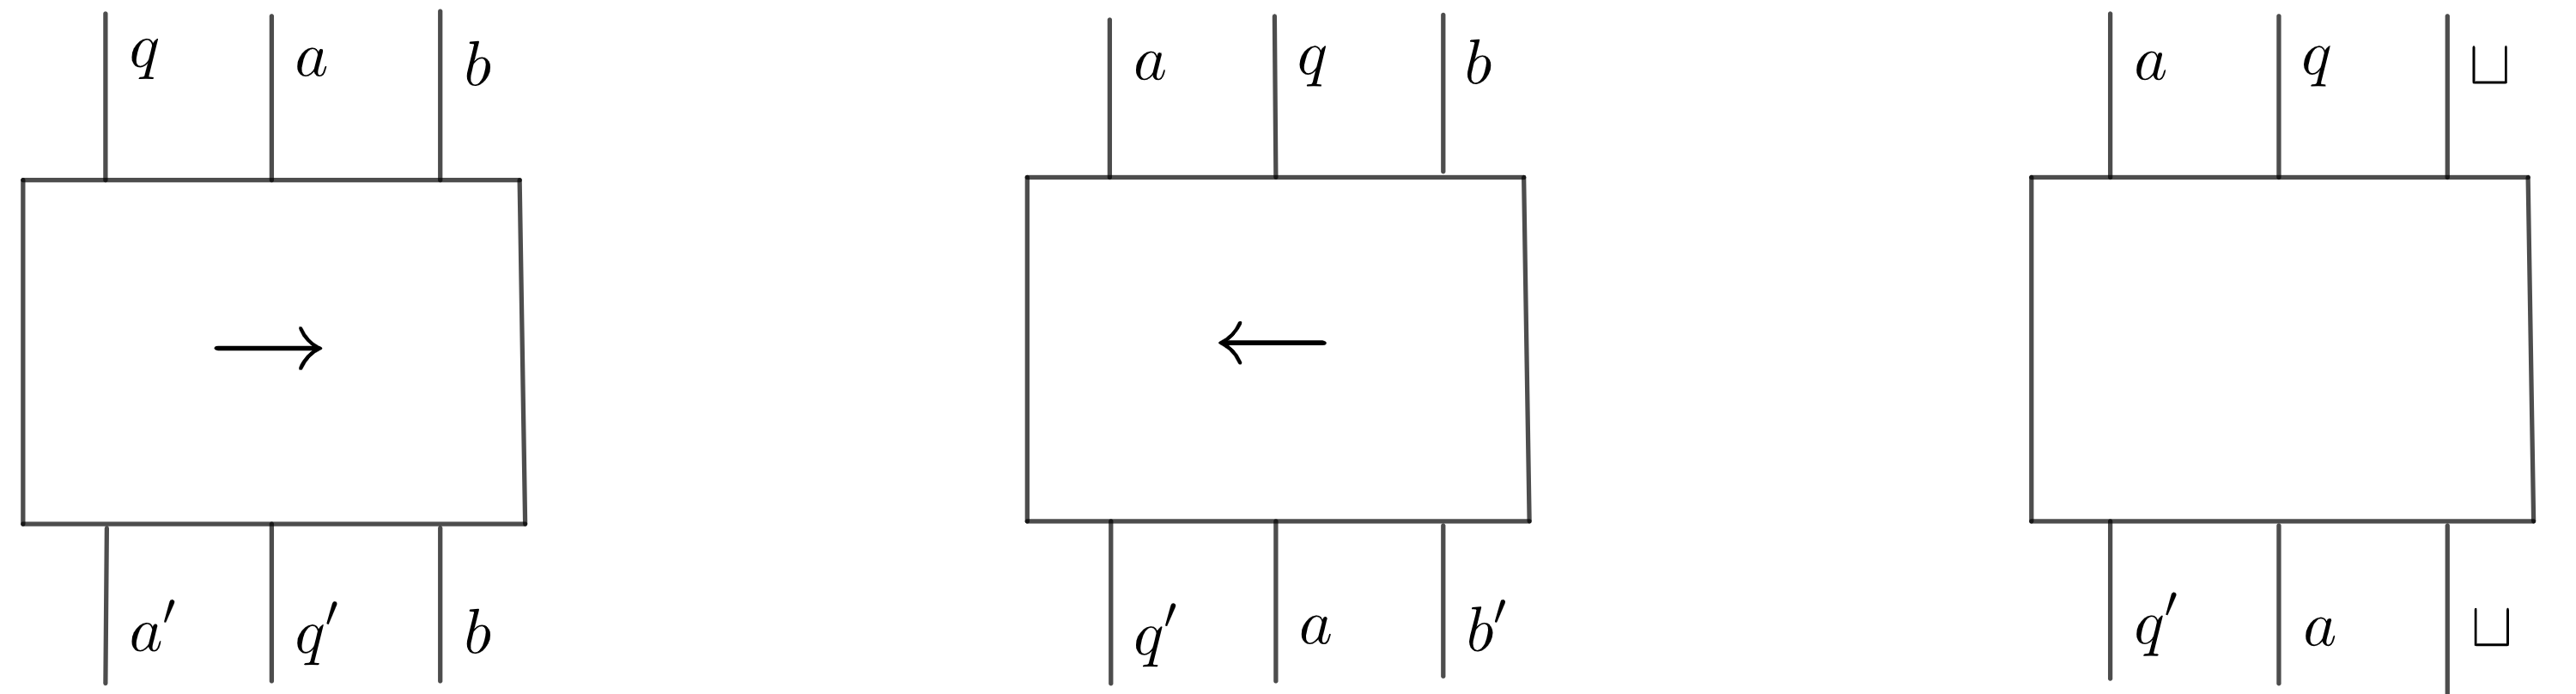
\includegraphics[scale=6.5]{diagrama/turing.png}
		\centering
	\end{figure}
	donde $a,a',b,b' \in \Sigma$, $q,q' \in Q$ tales que $\delta (q, a)=(q',a',\rightarrow)$, $\delta (q, b)=(q',b',\leftarrow)$ y $\delta (q, \sqcup)=(q',\sqcup,\rightarrow)$. Además, agregamos las reglas de producción $$x \to q_0 x \qquad \qquad \text{y} \qquad \qquad xsy \to s$$ 
    necesaria para inicializar la banda y para limpiarla. \\
	Veamos que $L=\mathcal{L}(G)$ \\
	Sea $w \in L$. Entonces $q_0w \vdash_M^* \alpha s \beta$. Pero notemos que para cada aplicación $\vdash_M$ tenemos un morfismo que actúa de la misma manera, entonces tenemos morfismos tales que
	\begin{center}
		\begin{tikzcd}
			q_0 w \arrow{r}{f_1}  & ...  \arrow{r}{f_n} & \alpha s \beta 
		\end{tikzcd}
	\end{center}
	Además como también tenemos las reglas de producción $w \to q_0w$ y $\alpha s \beta \to s$ tenemos una derivación $w \to s$ en $G$. Por lo tanto, $w \in \mathcal{L}(G)$ \\
	Para el regreso, sea $w \in \mathcal{L}(G)$, entonces existe una derivación $w \to s$. \\
	Observemos que por las reglas producción, tenemos la derivación es necesariamente de la siguiente forma
		\begin{center}
		\begin{tikzcd}
			w \arrow{r}  & q_0 w \arrow{r} & ...  \arrow{r} &  \alpha s \beta \arrow{r}  & s 
		\end{tikzcd}
		\end{center}
	Pero la derivación intermedia solo puede lograrse con reglas de producción de la forma $\leftarrow$ y $\rightarrow$, las cuales corresponden con derivaciones en $\vdash_M$, por lo tanto, $q_0 w \vdash_M^* \alpha w \beta$. Por lo tanto, $w \in L$.\\
	Por lo tanto, $L=\mathcal{L}(G)$
\end{proof}

Terminemos este capítulo con el siguiente ejemplo

\begin{ej}
	El lenguaje $L=\{ a^i b^i c^i | i \in \mathbb{N}\}$ no es regular, pero sí es recursivamente enumerable. \\
	Una máquina de Turing que acepte el lenguaje anterior es la siguiente: 
	
	\begin{tabular}{|c|c|c|c|c|c|c|c|}
		\hline
		$\delta$ & $a$ & $b$ & $c$ & $x$ & $y$ & $z$ & $\sqcup$  \\
		\hline
		$q_0$ & $q_1,x,\to$ &  &  &  & $q_4,y,\to$ &  & $q_5,\sqcup,\to$  \\
		\hline
		$q_1$ & $q_1,a,\to$ & $q_2,y,\to$ &  &  & $q_1,y,\to$ &  &    \\
		\hline
		$q_2$ &  & $q_2,b,\to$ & $q_3,z,\leftarrow$ &  &  & $q_2,z,\to$ &  \\
		\hline
		$q_3$ & $q_3,a,\leftarrow $ & $q_3,b,\leftarrow $ & $q_3,c,\leftarrow $ & $q_0,x,\to$ & $q_3,y,\leftarrow $ & $q_3,z,\leftarrow$ &    \\
		\hline
		$q_4$ &  &  &  &  & $q_4,y,\to$ & $q_4,z,\to$ & $q_5, \sqcup, \to$   \\
		\hline
		$q_5$ &  &  &  &  &  &  & $q_5,s,\to$ \\
		\hline
	\end{tabular}
	\\
    
    \noindent Veamos la derivación en la gramática monoidal asociada de la palabra $aabbcc$
\end{ej}
\newpage
\[
\begin{tikzcd}[scale=0.1, column sep=small, row sep=small, /tikz/execute at end picture={
        \node (large) [rectangle, draw, fit=(A1) (A2) (A3)] {};
        \node (large) [rectangle, draw, fit=(B1) (B2) (B3)] {};
        \node (large) [rectangle, draw, fit=(C1) (C2) (C3)] {};
        \node (large) [rectangle, draw, fit=(D1) (D2) (D3)] {};
        \node (large) [rectangle, draw, fit=(E1) (E2) (E3)] {};
        \node (large) [rectangle, draw, fit=(F1) (F2) (F3)] {};
        \node (large) [rectangle, draw, fit=(G1) (G2) (G3)] {};
        \node (large) [rectangle, draw, fit=(H1) (H2) (H3)] {};
        \node (large) [rectangle, draw, fit=(I1) (I2) (I3)] {};
        \node (large) [rectangle, draw, fit=(J1) (J2) (J3)] {};
        \node (large) [rectangle, draw, fit=(K1) (K2) (K3)] {};
    }]
    q_0 \arrow[no head, shorten >=7pt]{d}{} & a \arrow[no head, shorten >=4pt]{d}{} & a \arrow[no head, shorten >=7pt]{d}{} & b \arrow[no head]{dd}{} & b \arrow[no head]{dd}{} & c \arrow[no head]{dd}{} & c \arrow[no head]{dd}{} \\
    |[alias=A1]| \arrow[no head, shorten <=2pt]{d}{} & |[alias=A2]| \rightarrow  \arrow[no head, shorten <=2pt]{d}{} & |[alias=A3]|  \arrow[no head, shorten <=2pt]{d}{} & \ & \ & \ & \ \\
    x \arrow[no head]{dd}{} & q_1 \arrow[no head, shorten >=7pt]{d}{} & a \arrow[no head, shorten >=4pt]{d}{} & b \arrow[no head, shorten >=7pt]{d}{} & b \arrow[no head]{dd}{} & c \arrow[no head]{dd}{} & c \arrow[no head]{dd}{} \\
    \ & |[alias=B1]| \arrow[no head, shorten <=2pt]{d}{} & |[alias=B2]| \rightarrow  \arrow[no head, shorten <=2pt]{d}{} & |[alias=B3]|  \arrow[no head, shorten <=2pt]{d}{} & \ & \ & \ \\
    x \arrow[no head]{dd}{} & a \arrow[no head]{dd}{} & q_1 \arrow[no head, shorten >=7pt]{d}{} & b \arrow[no head, shorten >=4pt]{d}{} & b \arrow[no head, shorten >=7pt]{d}{} & c \arrow[no head]{dd}{} & c \arrow[no head]{dd}{} \\
    \ & \ & |[alias=C1]| \arrow[no head, shorten <=2pt]{d}{} & |[alias=C2]| \rightarrow  \arrow[no head, shorten <=2pt]{d}{} & |[alias=C3]|  \arrow[no head, shorten <=2pt]{d}{} & \ & \ \\
    x \arrow[no head]{dd}{} & a \arrow[no head]{dd}{} & y \arrow[no head]{dd}{} & q_2 \arrow[no head, shorten >=7pt]{d}{} & b \arrow[no head, shorten >=4pt]{d}{} & c \arrow[no head, shorten >=7pt]{d}{} & c \arrow[no head]{dd}{} \\
    \ & \ & \ & |[alias=D1]| \arrow[no head, shorten <=2pt]{d}{} & |[alias=D2]| \rightarrow  \arrow[no head, shorten <=2pt]{d}{} & |[alias=D3]|  \arrow[no head, shorten <=2pt]{d}{} & \ \\
    x \arrow[no head]{dd}{} & a \arrow[no head]{dd}{} & y \arrow[no head]{dd}{} & b \arrow[no head, shorten >=7pt]{d}{} & q_2 \arrow[no head, shorten >=4pt]{d}{} & c \arrow[no head, shorten >=7pt]{d}{} & c \arrow[no head]{dd}{} \\
    \ & \ & \ & |[alias=E1]| \arrow[no head, shorten <=2pt]{d}{} & |[alias=E2]| \leftarrow  \arrow[no head, shorten <=2pt]{d}{} & |[alias=E3]|  \arrow[no head, shorten <=2pt]{d}{} & \ \\
    x \arrow[no head]{dd}{} & a \arrow[no head]{dd}{} & y \arrow[no head, shorten >=7pt]{d}{} & q_3 \arrow[no head, shorten >=4pt]{d}{} & b \arrow[no head, shorten >=7pt]{d}{} & z \arrow[no head]{dd}{} & c \arrow[no head]{dd}{} \\
    \ & \ & |[alias=F1]| \arrow[no head, shorten <=2pt]{d}{} & |[alias=F2]| \leftarrow  \arrow[no head, shorten <=2pt]{d}{} & |[alias=F3]|  \arrow[no head, shorten <=2pt]{d}{} & \ & \ \\
    x \arrow[no head]{dd}{} & a \arrow[no head, shorten >=7pt]{d}{} & q_3 \arrow[no head, shorten >=4pt]{d}{} & y \arrow[no head, shorten >=7pt]{d}{} & b \arrow[no head]{dd}{} & z \arrow[no head]{dd}{} & c \arrow[no head]{dd}{} \\
    \ & |[alias=G1]| \arrow[no head, shorten <=2pt]{d}{} & |[alias=G2]| \leftarrow  \arrow[no head, shorten <=2pt]{d}{} & |[alias=G3]|  \arrow[no head, shorten <=2pt]{d}{} & \arrow[no head, shorten <=2pt]{d}{} & \ & \ \\
    x \arrow[no head, shorten >=7pt]{d}{} & q_3 \arrow[no head, shorten >=4pt]{d}{} & a \arrow[no head, shorten >=7pt]{d}{} & y \arrow[no head, shorten >=7pt]{dd}{} & b \arrow[no head]{dd}{} & z \arrow[no head]{dd}{} & c \arrow[no head]{dd}{} \\
    |[alias=H1]| \arrow[no head, shorten <=2pt]{d}{} & |[alias=H2]| \leftarrow  \arrow[no head, shorten <=2pt]{d}{} & |[alias=H3]|  \arrow[no head, shorten <=2pt]{d}{} &  \arrow[no head, shorten <=2pt]{d}{} & \arrow[no head, shorten <=2pt]{d}{} & \ & \ \\
    q_3 \arrow[no head, shorten >=7pt]{d}{} & x \arrow[no head, shorten >=4pt]{d}{} & a \arrow[no head, shorten >=7pt]{d}{} & y \arrow[no head, shorten >=7pt]{dd}{} & b \arrow[no head]{dd}{} & z \arrow[no head]{dd}{} & c \arrow[no head]{dd}{} \\
    |[alias=I1]| \arrow[no head, shorten <=2pt]{d}{} & |[alias=I2]| \rightarrow  \arrow[no head, shorten <=2pt]{d}{} & |[alias=I3]|  \arrow[no head, shorten <=2pt]{d}{} &  \arrow[no head, shorten <=2pt]{d}{} & \arrow[no head, shorten <=2pt]{d}{} & \ & \ \\
    x \arrow[no head]{dd}{} & q_0 \arrow[no head, shorten >=7pt]{d}{} & a \arrow[no head, shorten >=4pt]{d}{} & y \arrow[no head, shorten >=7pt]{d}{} & b \arrow[no head]{dd}{} & z \arrow[no head]{dd}{} & c \arrow[no head]{dd}{} \\
    & |[alias=J1]| \arrow[no head, shorten <=2pt]{d}{} & |[alias=J2]| \rightarrow  \arrow[no head, shorten <=2pt]{d}{} & |[alias=J3]| \ \arrow[no head, shorten <=2pt]{d}{} &  \arrow[no head, shorten <=2pt]{d}{} & \arrow[no head, shorten <=2pt]{d}{} & \ & \ \\
    x \arrow[no head]{dd}{} & x \arrow[no head]{dd}{} & q_1 \arrow[no head, shorten >=7pt]{d}{} & y \arrow[no head, shorten >=4pt]{d}{} & b \arrow[no head, shorten >=7pt]{d}{} & z \arrow[no head]{dd}{} & c \arrow[no head]{dd}{} \\
    \ \arrow[no head]{d}{} & \ \arrow[no head, shorten <=2pt]{d}{} & |[alias=K1]| \arrow[no head, shorten <=2pt]{d}{} & |[alias=K2]| \rightarrow  \arrow[no head, shorten <=2pt]{d}{} & |[alias=K3]|  \arrow[no head, shorten <=2pt]{d}{} & \ & \ \\
    x & x & y & q_1 & b & z & c
\end{tikzcd}
\]

\newpage

\[
\begin{tikzcd}[scale=0.1, column sep=small, row sep=small, /tikz/execute at end picture={
        \node (large) [rectangle, draw, fit=(A1) (A2) (A3)] {};
        \node (large) [rectangle, draw, fit=(B1) (B2) (B3)] {};
        \node (large) [rectangle, draw, fit=(C1) (C2) (C3)] {};
        \node (large) [rectangle, draw, fit=(D1) (D2) (D3)] {};
        \node (large) [rectangle, draw, fit=(E1) (E2) (E3)] {};
        \node (large) [rectangle, draw, fit=(F1) (F2) (F3)] {};
        \node (large) [rectangle, draw, fit=(G1) (G2) (G3)] {};
        \node (large) [rectangle, draw, fit=(H1) (H2) (H3)] {};
        \node (large) [rectangle, draw, fit=(I1) (I2) (I3)] {};
        \node (large) [rectangle, draw, fit=(J1) (J2) (J3)] {};
        \node (large) [rectangle, draw, fit=(K1) (K2)] {};
        \node (large) [rectangle, draw, fit=(L1)] {};
        \node (large) [rectangle, draw, fit=(M1) (M2)] {};
    }]
    x \arrow[no head]{dd}{} & x \arrow[no head]{dd}{} & y \arrow[no head]{dd}{} & q_1 \arrow[no head, shorten >=7pt]{d}{} & b \arrow[no head, shorten >=4pt]{d}{} & z \arrow[no head, shorten >=7pt]{d}{} & c \arrow[no head]{dd}{} \\
    \ \arrow[no head]{d}{} & \ \arrow[no head]{d}{} & \arrow[no head]{d}{} & |[alias=A1]| \arrow[no head, shorten <=2pt]{d}{} & |[alias=A2]| \rightarrow  \arrow[no head, shorten <=2pt]{d}{} & |[alias=A3]|  \arrow[no head, shorten <=2pt]{d}{} & \ \arrow[no head, shorten <=2pt]{d}{} \\
    x \arrow[no head]{dd}{} & x \arrow[no head]{dd}{} & y \arrow[no head]{dd}{} & y \arrow[no head]{dd}{} & q_2\arrow[no head, shorten >=7pt]{d}{} & z \arrow[no head, shorten >=4pt]{d}{} & c \arrow[no head, shorten >=7pt]{d}{} \\
    \ \arrow[no head]{d}{} & \ \arrow[no head]{d}{} & \arrow[no head]{d}{} & \arrow[no head]{d}{} & |[alias=B1]| \arrow[no head, shorten <=2pt]{d}{} & |[alias=B2]| \rightarrow  \arrow[no head, shorten <=2pt]{d}{} & |[alias=B3]|  \arrow[no head, shorten <=2pt]{d}{} \\
    x \arrow[no head]{dd}{} & x \arrow[no head]{dd}{} & y \arrow[no head]{dd}{} & y \arrow[no head]{dd}{} & z \arrow[no head, shorten >=7pt]{d}{} & q_2 \arrow[no head, shorten >=4pt]{d}{} & c \arrow[no head, shorten >=7pt]{d}{} \\
    \ \arrow[no head]{d}{} & \ \arrow[no head]{d}{} & \arrow[no head]{d}{} & \arrow[no head]{d}{} & |[alias=C1]| \arrow[no head, shorten <=2pt]{d}{} & |[alias=C2]| \leftarrow  \arrow[no head, shorten <=2pt]{d}{} & |[alias=C3]|  \arrow[no head, shorten <=2pt]{d}{} \\
    x \arrow[no head]{dd}{} & x \arrow[no head]{dd}{} & y \arrow[no head]{dd}{} & y \arrow[no head, shorten >=7pt]{d}{} & q_3 \arrow[no head, shorten >=4pt]{d}{} & z \arrow[no head, shorten >=7pt]{d}{} & z \arrow[no head]{dd}{} \\
    \ \arrow[no head]{d}{} & \ \arrow[no head]{d}{} & \arrow[no head]{d}{} & |[alias=D1]| \arrow[no head, shorten <=2pt]{d}{} & |[alias=D2]| \leftarrow  \arrow[no head, shorten <=2pt]{d}{} & |[alias=D3]|  \arrow[no head, shorten <=2pt]{d}{} & \ \arrow[no head]{d}{} \\
    x \arrow[no head]{dd}{} & x \arrow[no head]{dd}{} & y \arrow[no head, shorten >=7pt]{d}{} & q_3 \arrow[no head, shorten >=4pt]{d}{} & y \arrow[no head, shorten >=7pt]{d}{} & z \arrow[no head]{dd}{} & z \arrow[no head]{dd}{} \\
    \ \arrow[no head]{d}{} & \ \arrow[no head]{d}{} & |[alias=E1]| \arrow[no head, shorten <=2pt]{d}{} & |[alias=E2]| \leftarrow  \arrow[no head, shorten <=2pt]{d}{} & |[alias=E3]|  \arrow[no head, shorten <=2pt]{d}{} & \arrow[no head]{d}{} & \ \arrow[no head]{d}{} \\
    x \arrow[no head]{dd}{} & x \arrow[no head, shorten >=7pt]{d}{} & q_3 \arrow[no head, shorten >=4pt]{d}{} & y \arrow[no head, shorten >=7pt]{d}{} & y \arrow[no head]{dd}{} & z \arrow[no head]{dd}{} & z \arrow[no head]{dd}{} \\
    \ \arrow[no head]{d}{} & |[alias=F1]| \arrow[no head, shorten <=2pt]{d}{} & |[alias=F2]| \leftarrow  \arrow[no head, shorten <=2pt]{d}{} & |[alias=F3]|  \arrow[no head, shorten <=2pt]{d}{} & \arrow[no head]{d}{} & \arrow[no head]{d}{} & \ \arrow[no head]{d}{} \\
    x \arrow[no head]{dd}{} & q_0 \arrow[no head, shorten >=7pt]{d}{} & x \arrow[no head, shorten >=4pt]{d}{} & y \arrow[no head, shorten >=7pt]{d}{} & y \arrow[no head]{dd}{} & z \arrow[no head]{dd}{} & z \arrow[no head]{dd}{} \\
    \ \arrow[no head]{d}{} & |[alias=G1]| \arrow[no head, shorten <=2pt]{d}{} & |[alias=G2]| \rightarrow  \arrow[no head, shorten <=2pt]{d}{} & |[alias=G3]|  \arrow[no head, shorten <=2pt]{d}{} & \arrow[no head]{d}{} & \arrow[no head]{d}{} & \ \arrow[no head]{d}{} \\
    x \arrow[no head]{dd}{} & x \arrow[no head]{dd}{} & q_1 \arrow[no head, shorten >=7pt]{d}{} & y \arrow[no head, shorten >=4pt]{d}{} & y \arrow[no head, shorten >=7pt]{d}{} & z \arrow[no head]{dd}{} & z \arrow[no head]{dd}{} \\
    \ \arrow[no head]{d}{} & \ \arrow[no head]{d}{} & |[alias=H1]| \arrow[no head, shorten <=2pt]{d}{} & |[alias=H2]| \rightarrow  \arrow[no head, shorten <=2pt]{d}{} & |[alias=H3]|  \arrow[no head, shorten <=2pt]{d}{} & \arrow[no head]{d}{} & \ \arrow[no head]{d}{} \\
    x \arrow[no head]{dd}{} & x \arrow[no head]{dd}{} & y \arrow[no head]{dd}{} & q_4 \arrow[no head, shorten >=7pt]{d}{} & y \arrow[no head, shorten >=4pt]{d}{} & z \arrow[no head, shorten >=7pt]{d}{} & z \arrow[no head]{dd}{} \\
    \ \arrow[no head]{d}{} & \ \arrow[no head]{d}{} & \arrow[no head]{d}{} & |[alias=I1]| \arrow[no head, shorten <=2pt]{d}{} & |[alias=I2]| \rightarrow  \arrow[no head, shorten <=2pt]{d}{} & |[alias=I3]|  \arrow[no head, shorten <=2pt]{d}{} & \ \arrow[no head]{d}{} \\
    x \arrow[no head]{dd}{} & x \arrow[no head]{dd}{} & y \arrow[no head]{dd}{} & y \arrow[no head]{dd}{} & q_4 \arrow[no head, shorten >=7pt]{d}{} & z \arrow[no head, shorten >=4pt]{d}{} & z \arrow[no head, shorten >=7pt]{d}{} \\
    \ \arrow[no head]{d}{} & \ \arrow[no head]{d}{} & \arrow[no head]{d}{} & \arrow[no head]{d}{} & |[alias=J1]| \arrow[no head, shorten <=2pt]{d}{} & |[alias=J2]| \rightarrow  \arrow[no head, shorten <=2pt]{d}{} & |[alias=J3]|  \arrow[no head, shorten <=2pt]{d}{} \\
    x \arrow[no head]{dd}{} & x \arrow[no head]{dd}{} & y \arrow[no head]{dd}{} & y \arrow[no head]{dd}{} & z \arrow[no head]{dd}{} & q_4 \arrow[no head, shorten >=7pt]{d}{} & z \arrow[no head, shorten >=4pt]{d}{} \\
    \ \arrow[no head]{d}{} & \ \arrow[no head]{d}{} & \arrow[no head]{d}{} & \arrow[no head]{d}{} & \arrow[no head]{d}{} & |[alias=K1]| \arrow[no head, shorten <=2pt]{d}{} & |[alias=K2]| \rightarrow  \arrow[no head, shorten <=2pt]{d}{} \\
    x \arrow[no head]{dd}{} & x \arrow[no head]{dd}{} & y \arrow[no head]{dd}{} & y \arrow[no head]{dd}{} & z \arrow[no head]{dd}{} & z \arrow[no head]{dd}{} & q_4 \arrow[no head, shorten >=4pt]{d}{} \\
    \ \arrow[no head]{d}{} & \ \arrow[no head]{d}{} & \arrow[no head]{d}{} & \arrow[no head]{d}{} & \arrow[no head]{d}{} & \arrow[no head]{d}{} & |[alias=L1]| \arrow[no head, shorten <=2pt]{d}{} \\
    x \arrow[no head, shorten >=4pt]{d}{}  & x \arrow[no head, shorten >=4pt]{d}{}  & y \arrow[no head, shorten >=4pt]{d}{}  & y \arrow[no head, shorten >=4pt]{d}{} & z \arrow[no head, shorten >=4pt]{d}{} & z \arrow[no head, shorten >=4pt]{d}{} & q_5 \arrow[no head, shorten >=4pt]{d}{}  \\
    |[alias=M1]| & \ & \ & \ & \ & \ & |[alias=M2]| \ \arrow[no head, shorten <=2pt]{d}{} \\
    \ & \ & \ & \ & \ & \ & s
\end{tikzcd}
\]














\end{document}